\documentclass[master.tex]{subfiles}
 
\newcommand{\meanxy}[1]{\left<#1\right>_{z,y}}
\newcommand{\Tflow}[0]{\overline{\Gamma}}

\begin{document}



\chapter{Effect of Polarization Equation Linearizations on tokamak edge turbulence}\label{sec:polarization_equation_evaluation}

\section{Introduction}
In both gyrokinetic and gyrofluid models the polarization equation plays a central role and the nonlinear nature is often approximated because of the large computational effort associated with the numerical schemes and the assumption that the amplitudes of turbulent fluctuations are much smaller than the background. This may hold for the core plasma but certainly not for the edge region where high background gradients are observed which lead to relatively high amplitude fluctuations if dense \textit{material} is transported from the core region of the separatrix into the \ac{SOL}. For instance the GYSELA polarization equation assumes a equilibrium density $n_0(r)$ where $r$ is to be identified with the $x$-direction \cite{GYSELACODE}. This comes close to linearization 3. The XGC1 code uses a similar approach \cite{XGC1Code}. The following results should give some insight on the effects of the different linearizations. It should be noted that this is not an extensive parameter study and considering the amount of parameters (>10) there could exist various other effects that are not represented by the particular parameters used in the following evaluation.

% The GENE code evaluates the non-linearity but the authors claim that it only has an effect if the electron Debye length $\lambda_{De}$ is comparable to the electron gyro radius $\rho_e$ which in a tokamak is not the case.

\section{Simulation Setup}

The evaluation of the linearizations is done on a 8x128x512 grid with $h_x$ and $h_y=1.0$. Two parameter sets are tested. The following parameter set is used for the first set and is the evaluation techniques are introduced:
\begin{itemize}
    \item $\Delta t$: 0.025
    \item $\hat{c}$: 5.0
    \item $\hat{\epsilon}$: 27000.0
    \item $mcv$: 0.02
    \item $magnetic Shear$: 1.2
    \item $\nu_{\parallel}$: 0.11
    \item $\nu_{\perp}$: 0.11
    \item core Density: 1.5
    \item edge Density: 0.13
\end{itemize}
The simulation is run on \ac{TV} node using the GPU implementations of the \ac{SOR}-solver and gyroaveraging operator. The lower resolution grid has been run for 200.000 iterations and a state snapshot is taken every 20,000 iterations.

\section{Equilibrium State}
At first the simulation develops strong turbulence and high fluctuations which result in an outburst of "material" (i. e. the total density decreases). Afterwards the simulation approaches a steady state where the state variables only vary little and a typical energy cascade forms. This equilibrium behavior can be seen by looking for instance at temporal evolution of the parallel kinetic energy (\autoref{sec:polar_parallel_velocities}) or the total density both restricted to the core and \ac{SOL} plasma (in/out separatrix) . The data suggests that a stable regime is reached after about 80,000 iterations. The idea now is to compare mean values over the simulation time where a equilibrium state has been reached. 

\begin{figure}[!hbtp]
    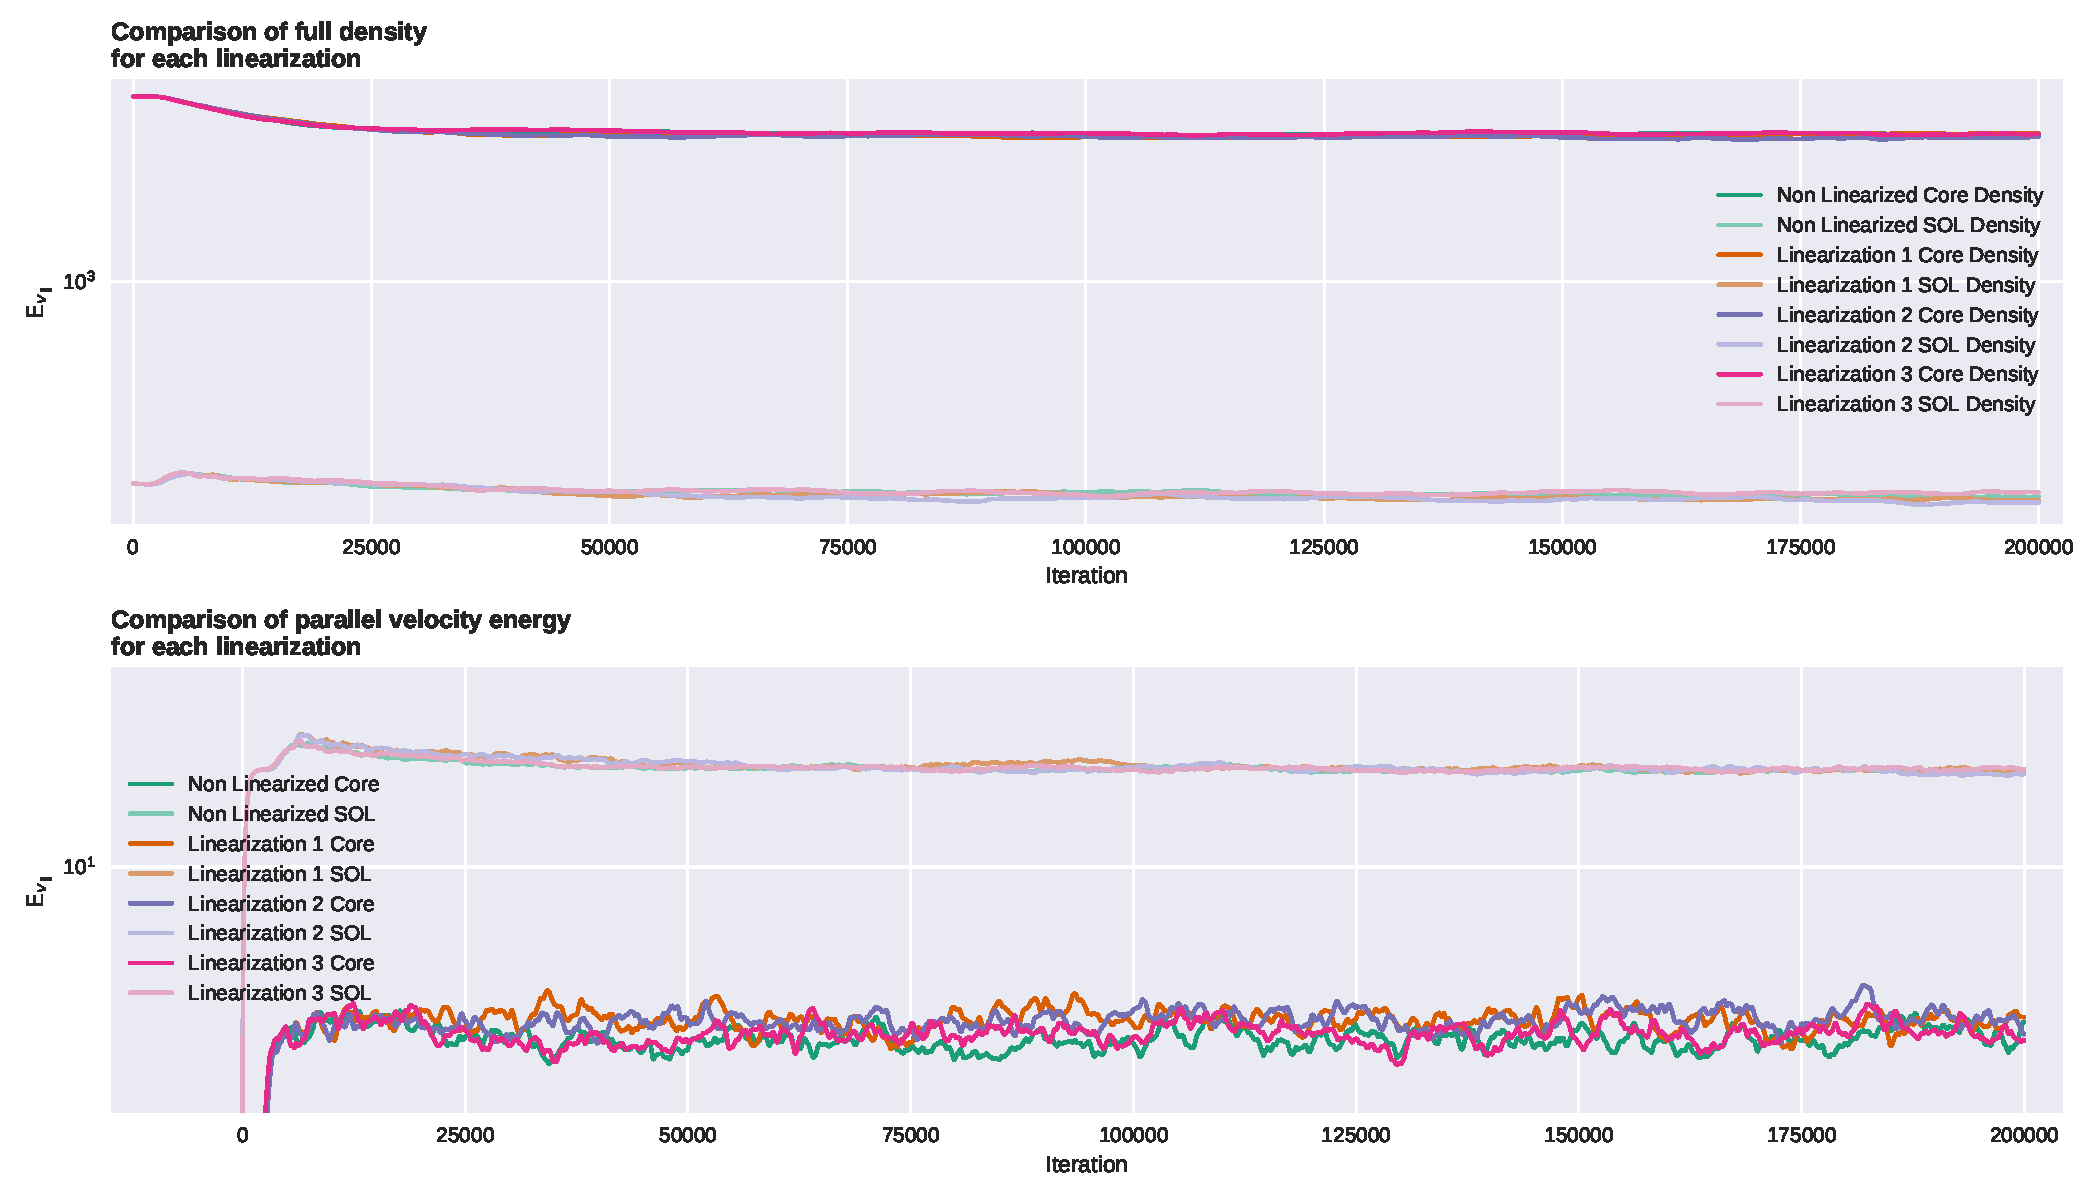
\includegraphics[width=\linewidth]{pdfs/equilibrium_state_low.pdf}
    \caption{Temporal evolution of ($E_n$ \autoref{sec:fluid-dynamics}) and the parallel kinetic energy (see \autoref{sec:polar_parallel_velocities}) both restricted to Core and \ac{SOL} region. After 80,000 iterations a steady state is reached.}
\end{figure}


\begin{blockquote}
    The errors attached to the mean values are calculated via the standard derivation but do not represent the error of multiple simulations or the response to disturbed input parameters but rather give an idea about the size of fluctuations in the equilibrium state.
\end{blockquote}
    
\section{Evaluation}
To compare the different linearizations defined in \autoref{sec:polarization-linearizations} the mean turbulent flow in the steady state regime is compared for the core and \ac{SOL} plasma. Further on the zonal potential  $\meanxy{\phi_e}$, the zonal flow ($\partial_x \meanxy{\phi_e}$) and the vorticity also defined as zonal flow potential ($\partial_{xx}\meanxy{\phi_e}$) are compared and finally the parallel velocity is taken into account.




\section{Turbulent Flow}
The turbulent flow is calculated as it is defined in \autoref{sec:simulation_quantities}. The turbulent flows (Core/\ac{SOL}) for the whole simulation are displayed in \autoref{fig:turbulent-flow-low} on a semi logarithmic grid. From this figure one can already see that there is no apparent difference for the turbulent flows in regard to the linearizations for this particular dataset.
\begin{figure}[!htbp]
    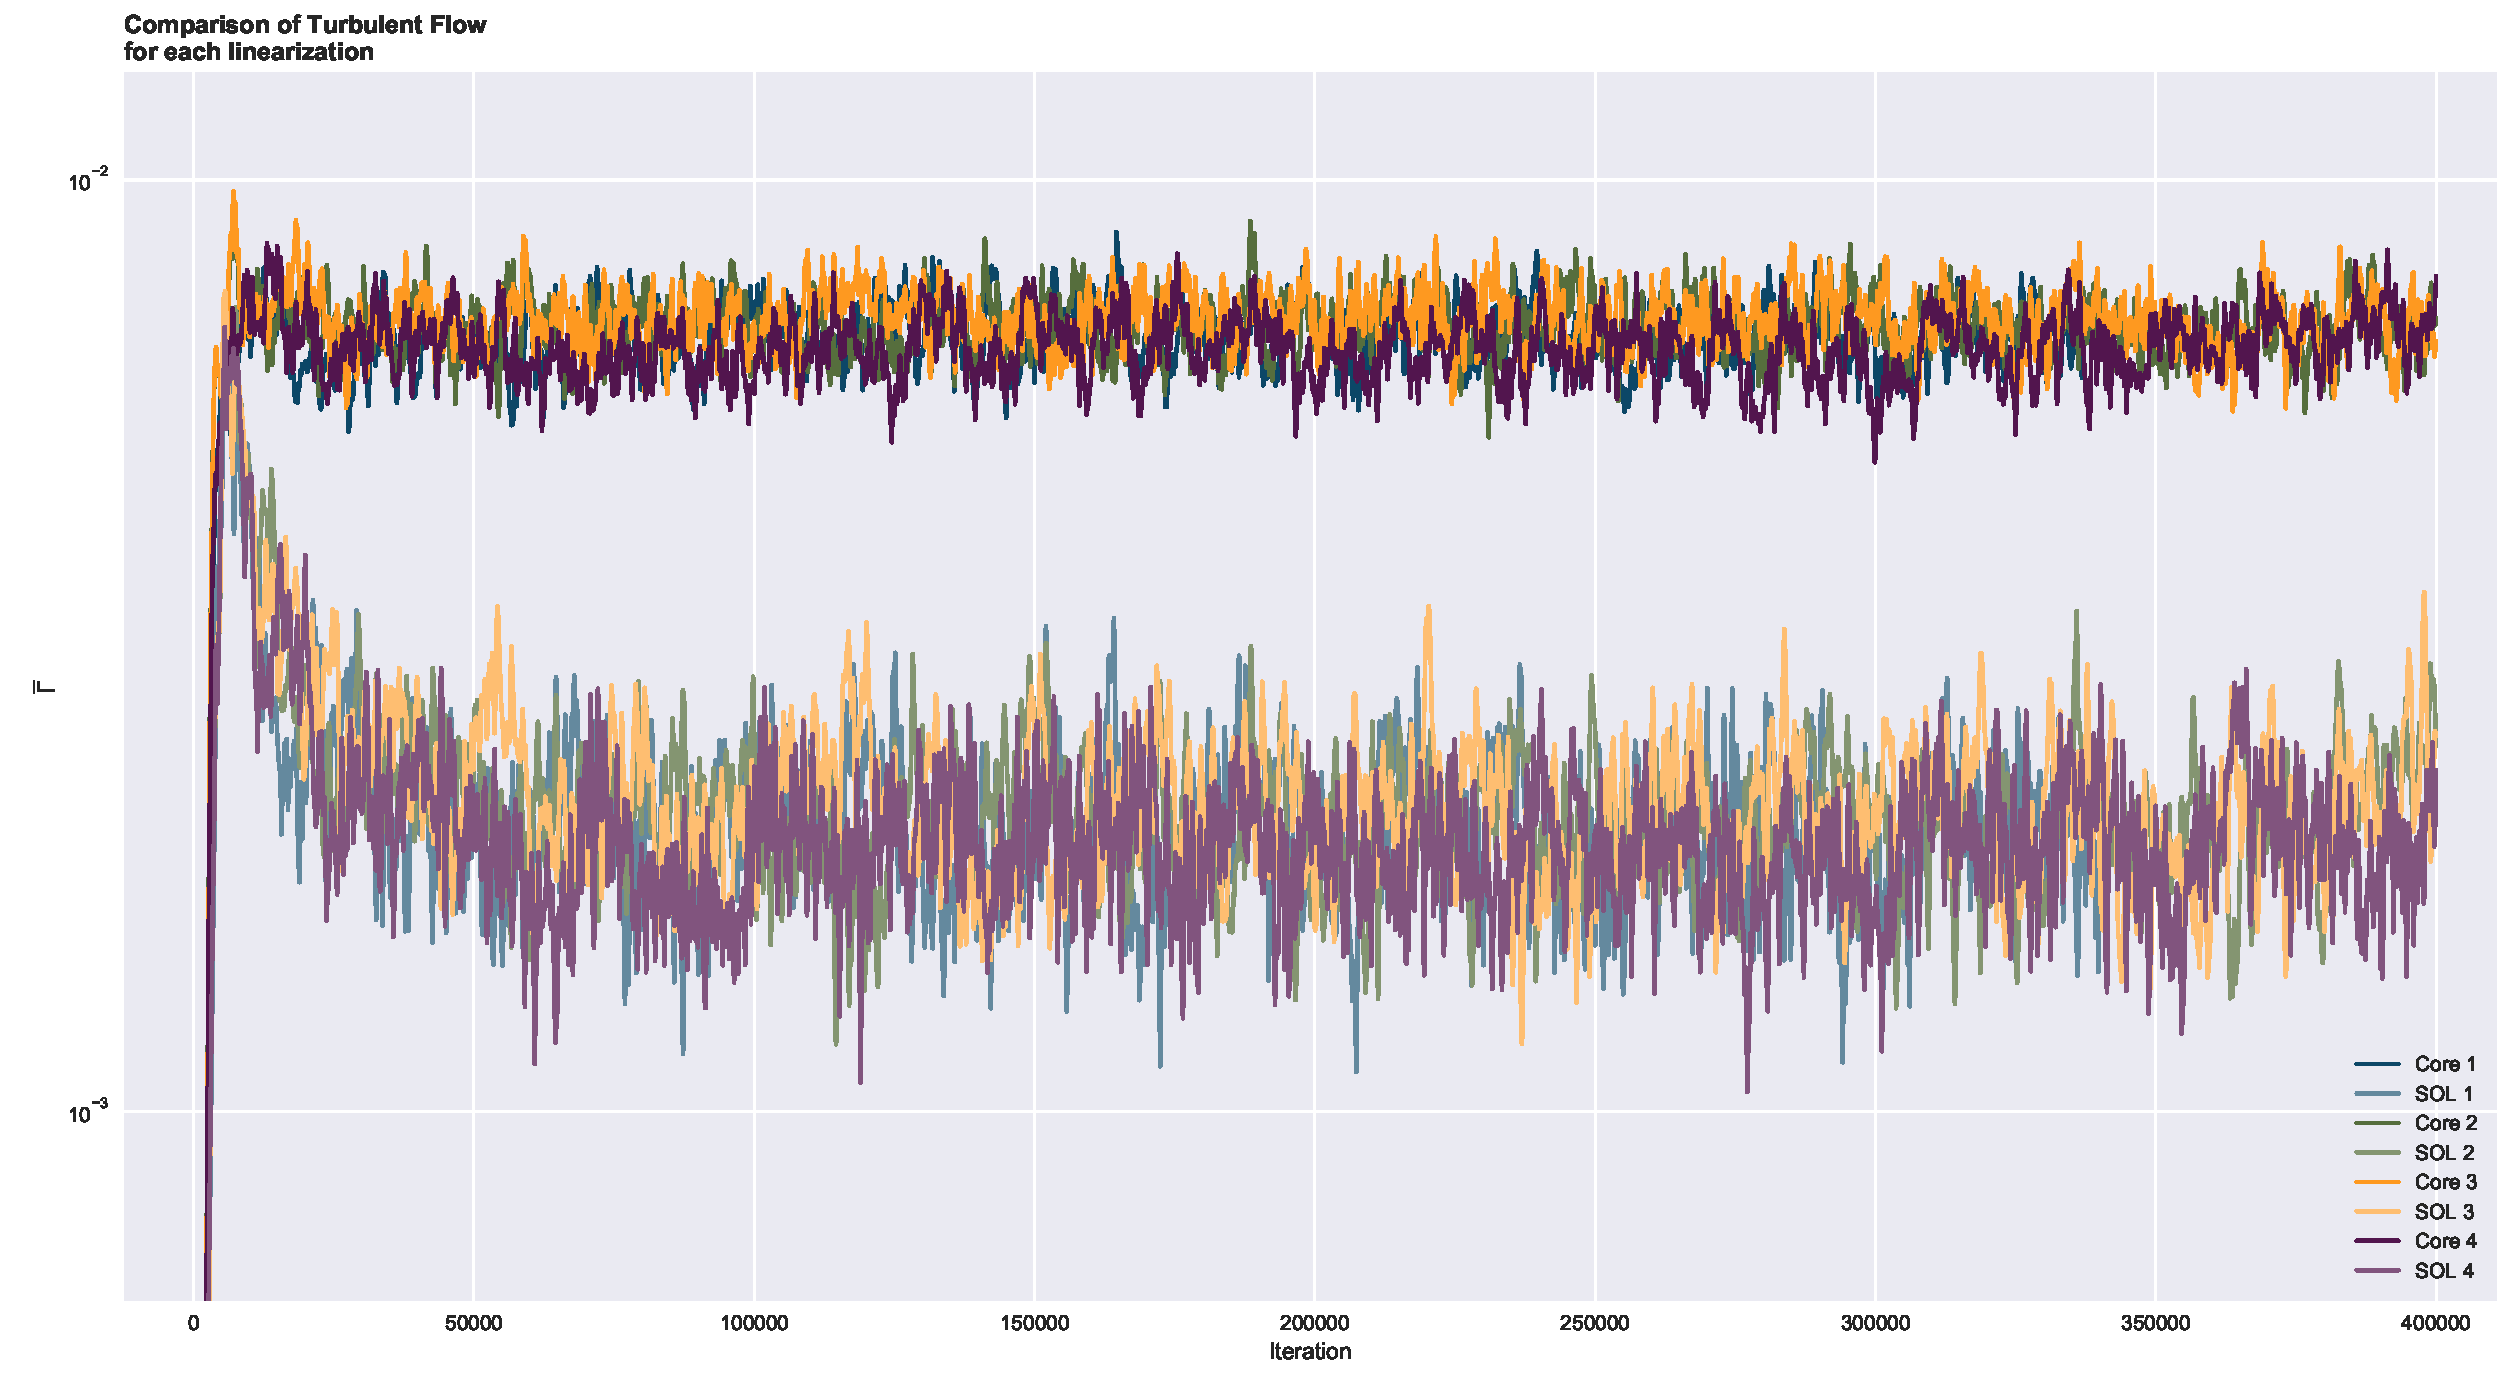
\includegraphics[width=\linewidth]{pdfs/turbulent-flow-low.pdf}
    \caption{Turbulent flow split into Core and \ac{SOL} region for each linearization. The lighter colors represent the \ac{SOL} parts.}
    \label{fig:turbulent-flow-low}
\end{figure}
\autoref{fig:turbulent-flow-low-means} shows the mean value of $\Tflow_{Core}$ and $\Tflow_{SOL}$ from 80,000 to 200,000 iterations. There may be a small indication that $\Tflow_{Core}$ is a little higher for the constant background (local model) linearizations but considering the magnitude of fluctuations (visualized by the error bars) this seems very far fetched. 



\begin{figure}[!htbp]
    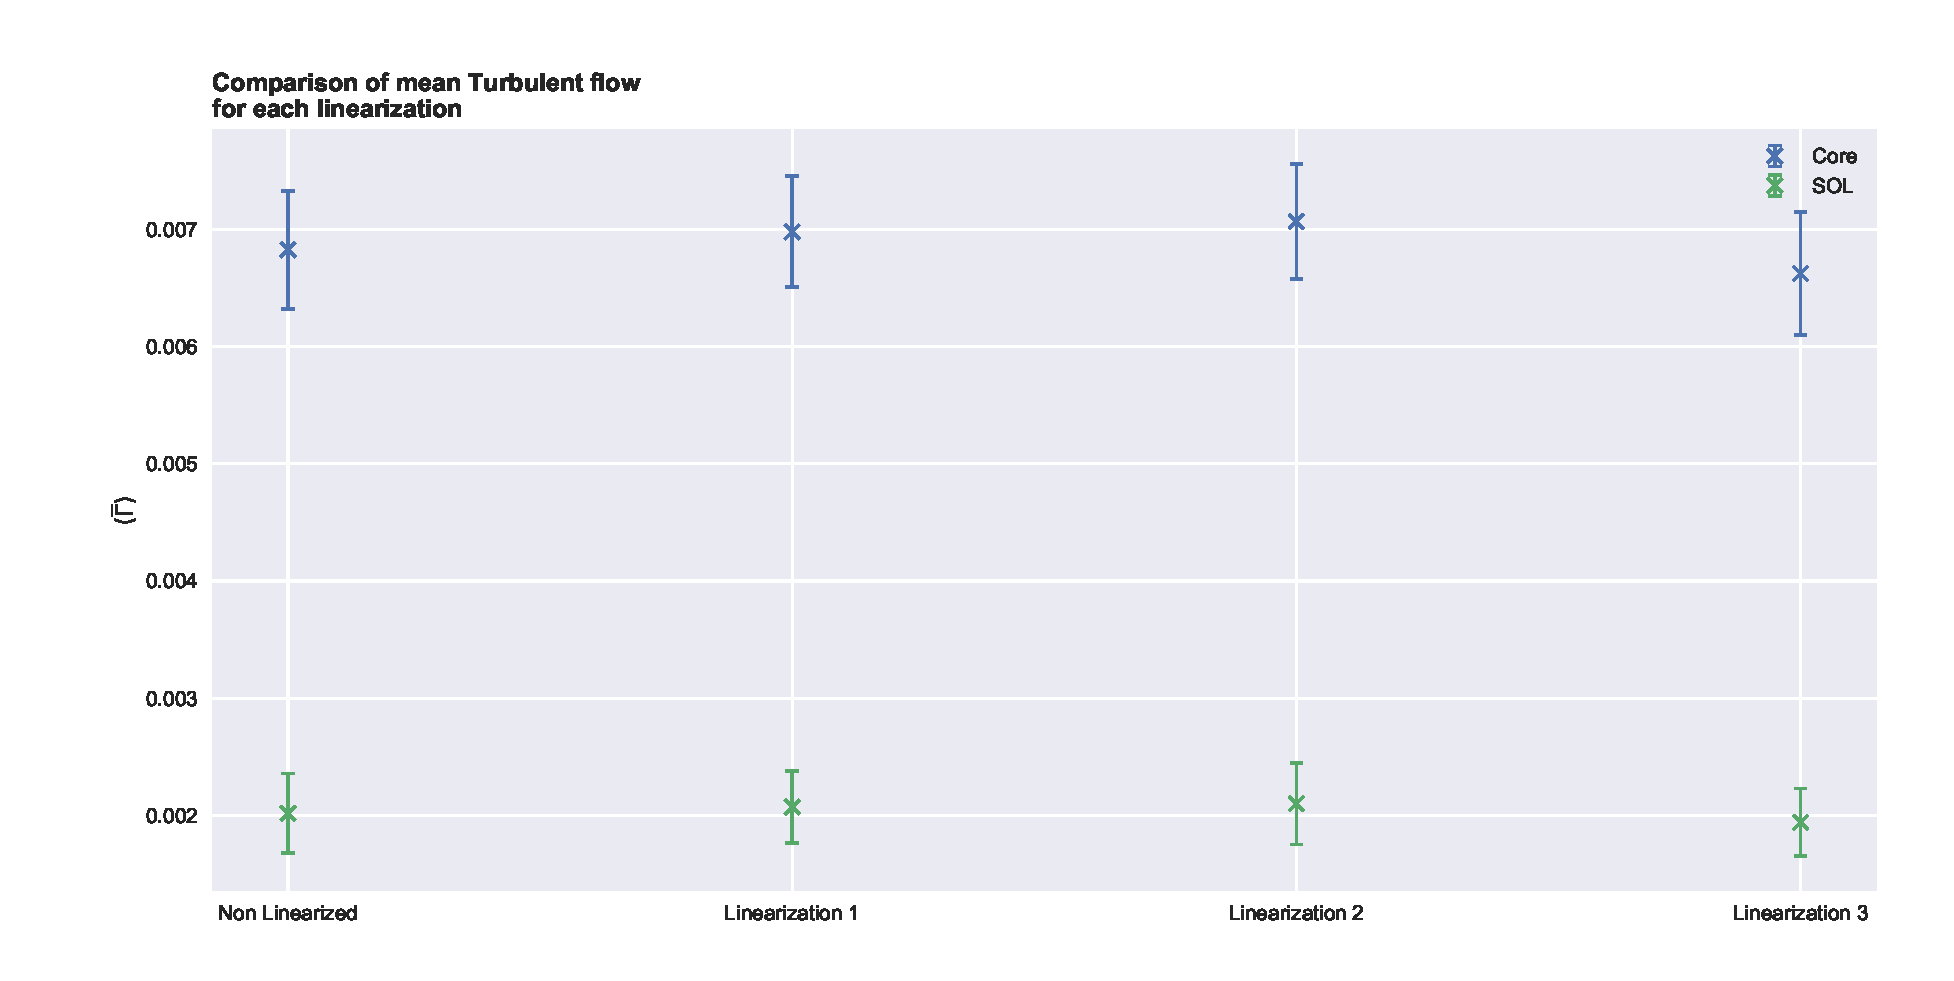
\includegraphics[width=\linewidth]{pdfs/turbulent-flow-low-means.pdf}
    \caption{Mean values of $\Tflow$ after 80,000 iterations. There is no apparent difference visible.}
    \label{fig:turbulent-flow-low-means}
\end{figure}

\section{Zonal Potential}

The same procedure of the previous section is applied to the zonal potential, zonal flow and zonal flow potential (vorticity). The results are shown in \autoref{fig:zonal-potential-low-all}.\\
They form two groups: The non linearized model and the third linearization share distinct features as well as the first and the second. Since the linearization specifically targets the gradient of the densities which is the strongest close to the core plasma, the greatest difference between the linearizations and the non linearized model is observed there. One has to note that on the boundaries numerical artifacts play a major role leading to artificial density gradients explaining for instance the \textit{bump} on the $x_L$ boundary. Looking at the zonal flow the first group generally produces a lower zonal flow away from the boundaries.

\begin{figure}[!htbp]
    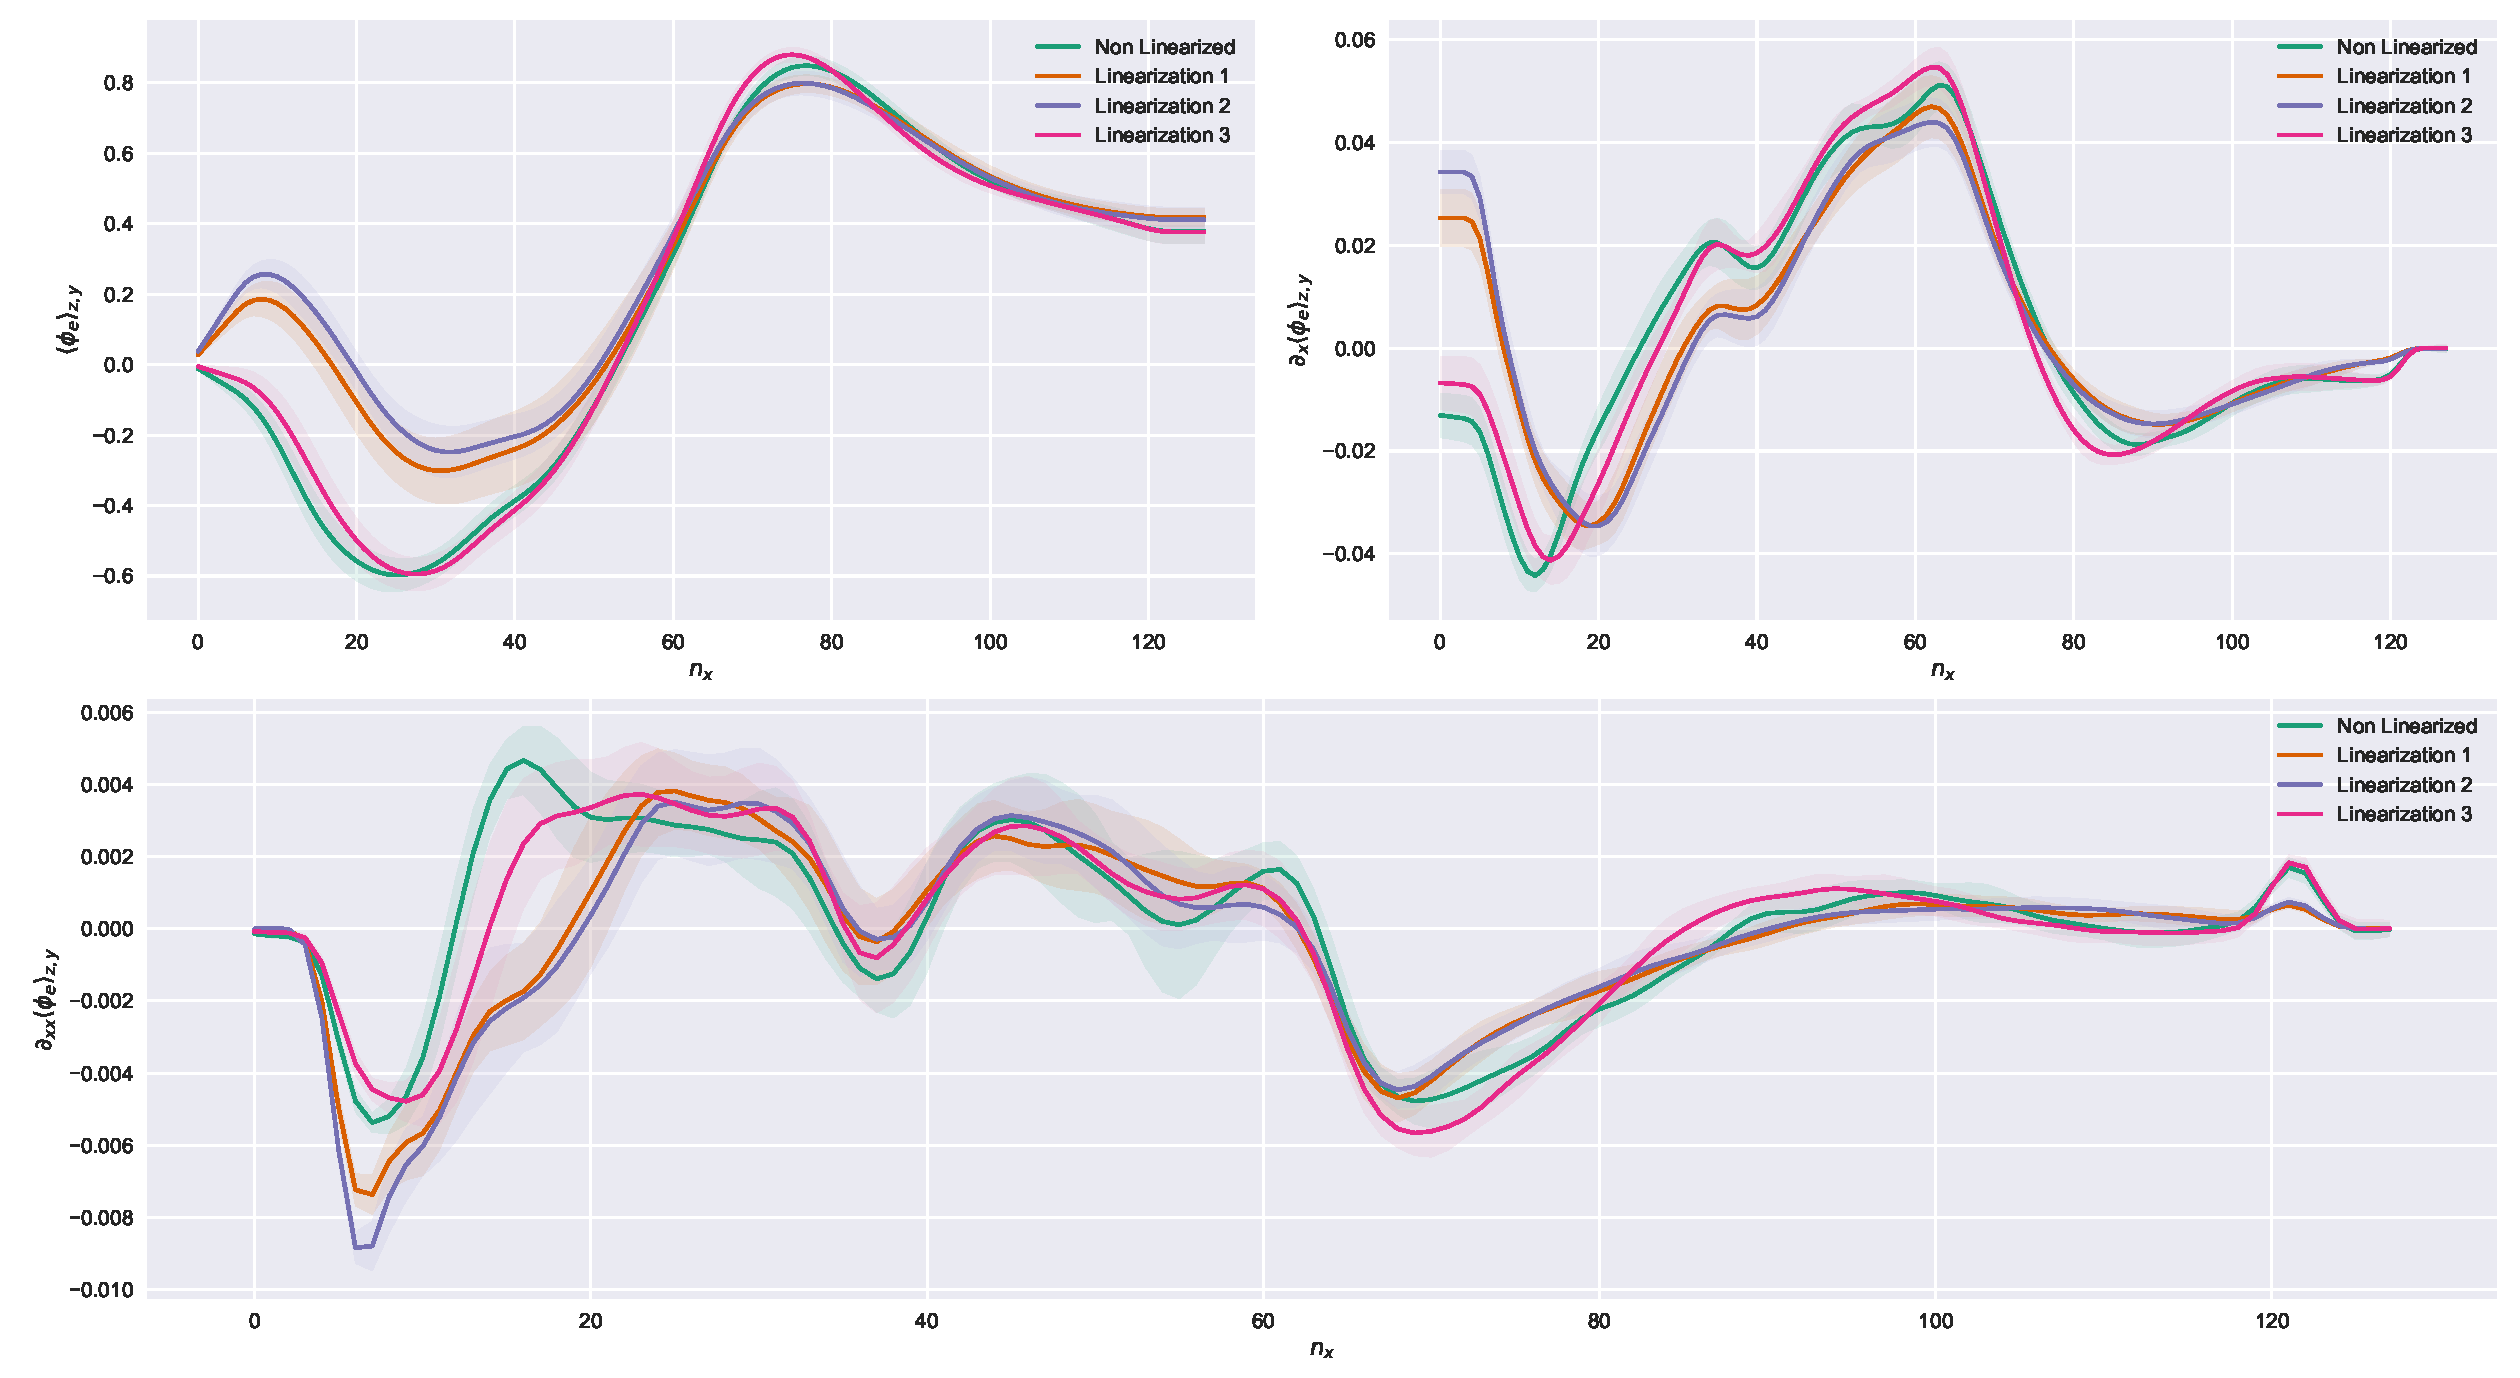
\includegraphics[width=\linewidth]{pdfs/zonal_potential_low.pdf}
    \caption{Mean values of Zonal Potential, Zonal Flow and Zonal Flow Potential of iteration 80,000-200,000. The shaded areas show fluctuations for each case.}
    \label{fig:zonal-potential-low-all}
\end{figure}

\section{Parallel Velocities}\label{sec:polar_parallel_velocities}

Something that is closely connected to the parallel kinetic energy of the system can be defined by:
\begin{equation}
    \mathrm{E}_{v_\parallel} = \hat{\epsilon} \cdot \int_{[z,x,y]} \left( \mu_ev_{e\parallel}^2 + \mu_iv_{i\parallel }^2 \right) \, dxdydz
\end{equation}
As in the previous chapters the integration will be restricted to either Core or the \ac{SOL} region. The time evolution of these quantities is shown in \autoref{fig:velocity-energy-low}.

\begin{figure}[!htbp]
    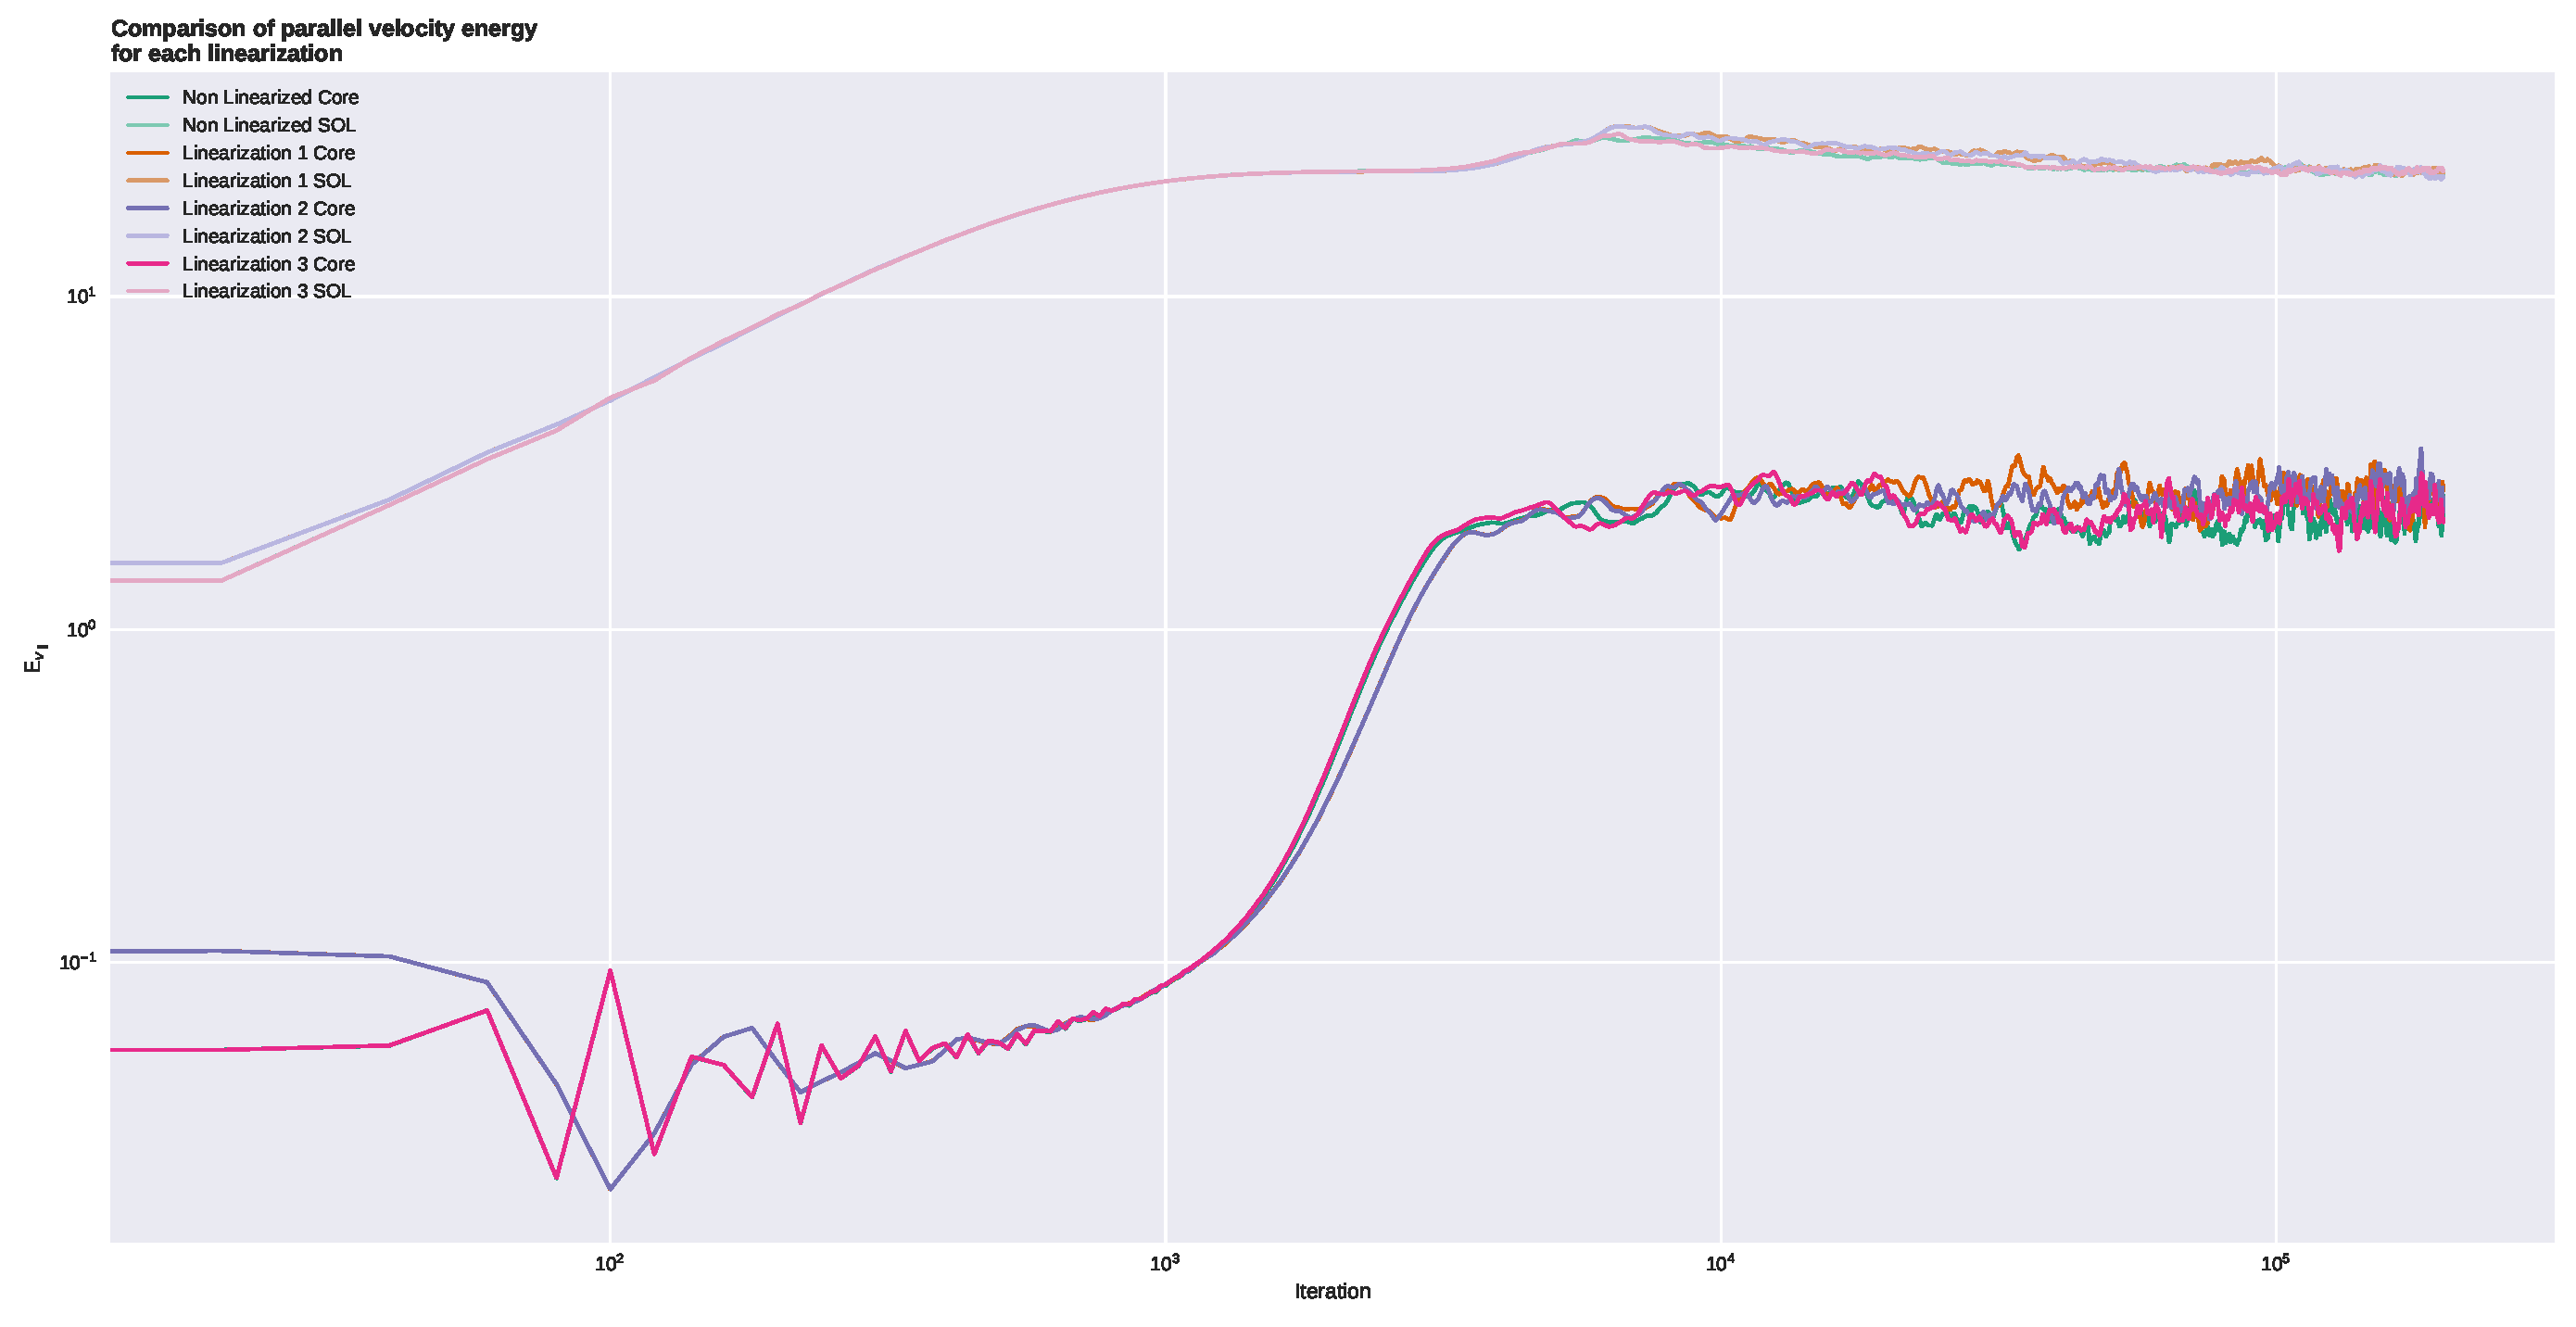
\includegraphics[width=\linewidth]{pdfs/velocity-energy-low.pdf}
    \caption{Time evolution of $\mathrm{E}_{v_\parallel}$ for Core and \ac{SOL} region. This time in a log-log coordinate system.}
    \label{fig:velocity-energy-low}
\end{figure}

The comparison shows no major difference but if one looks at the mean values the splitting into two groups from the previous section is visible again (\autoref{fig:velocity-energy-low-mean}).


\begin{figure}[!htbp]
    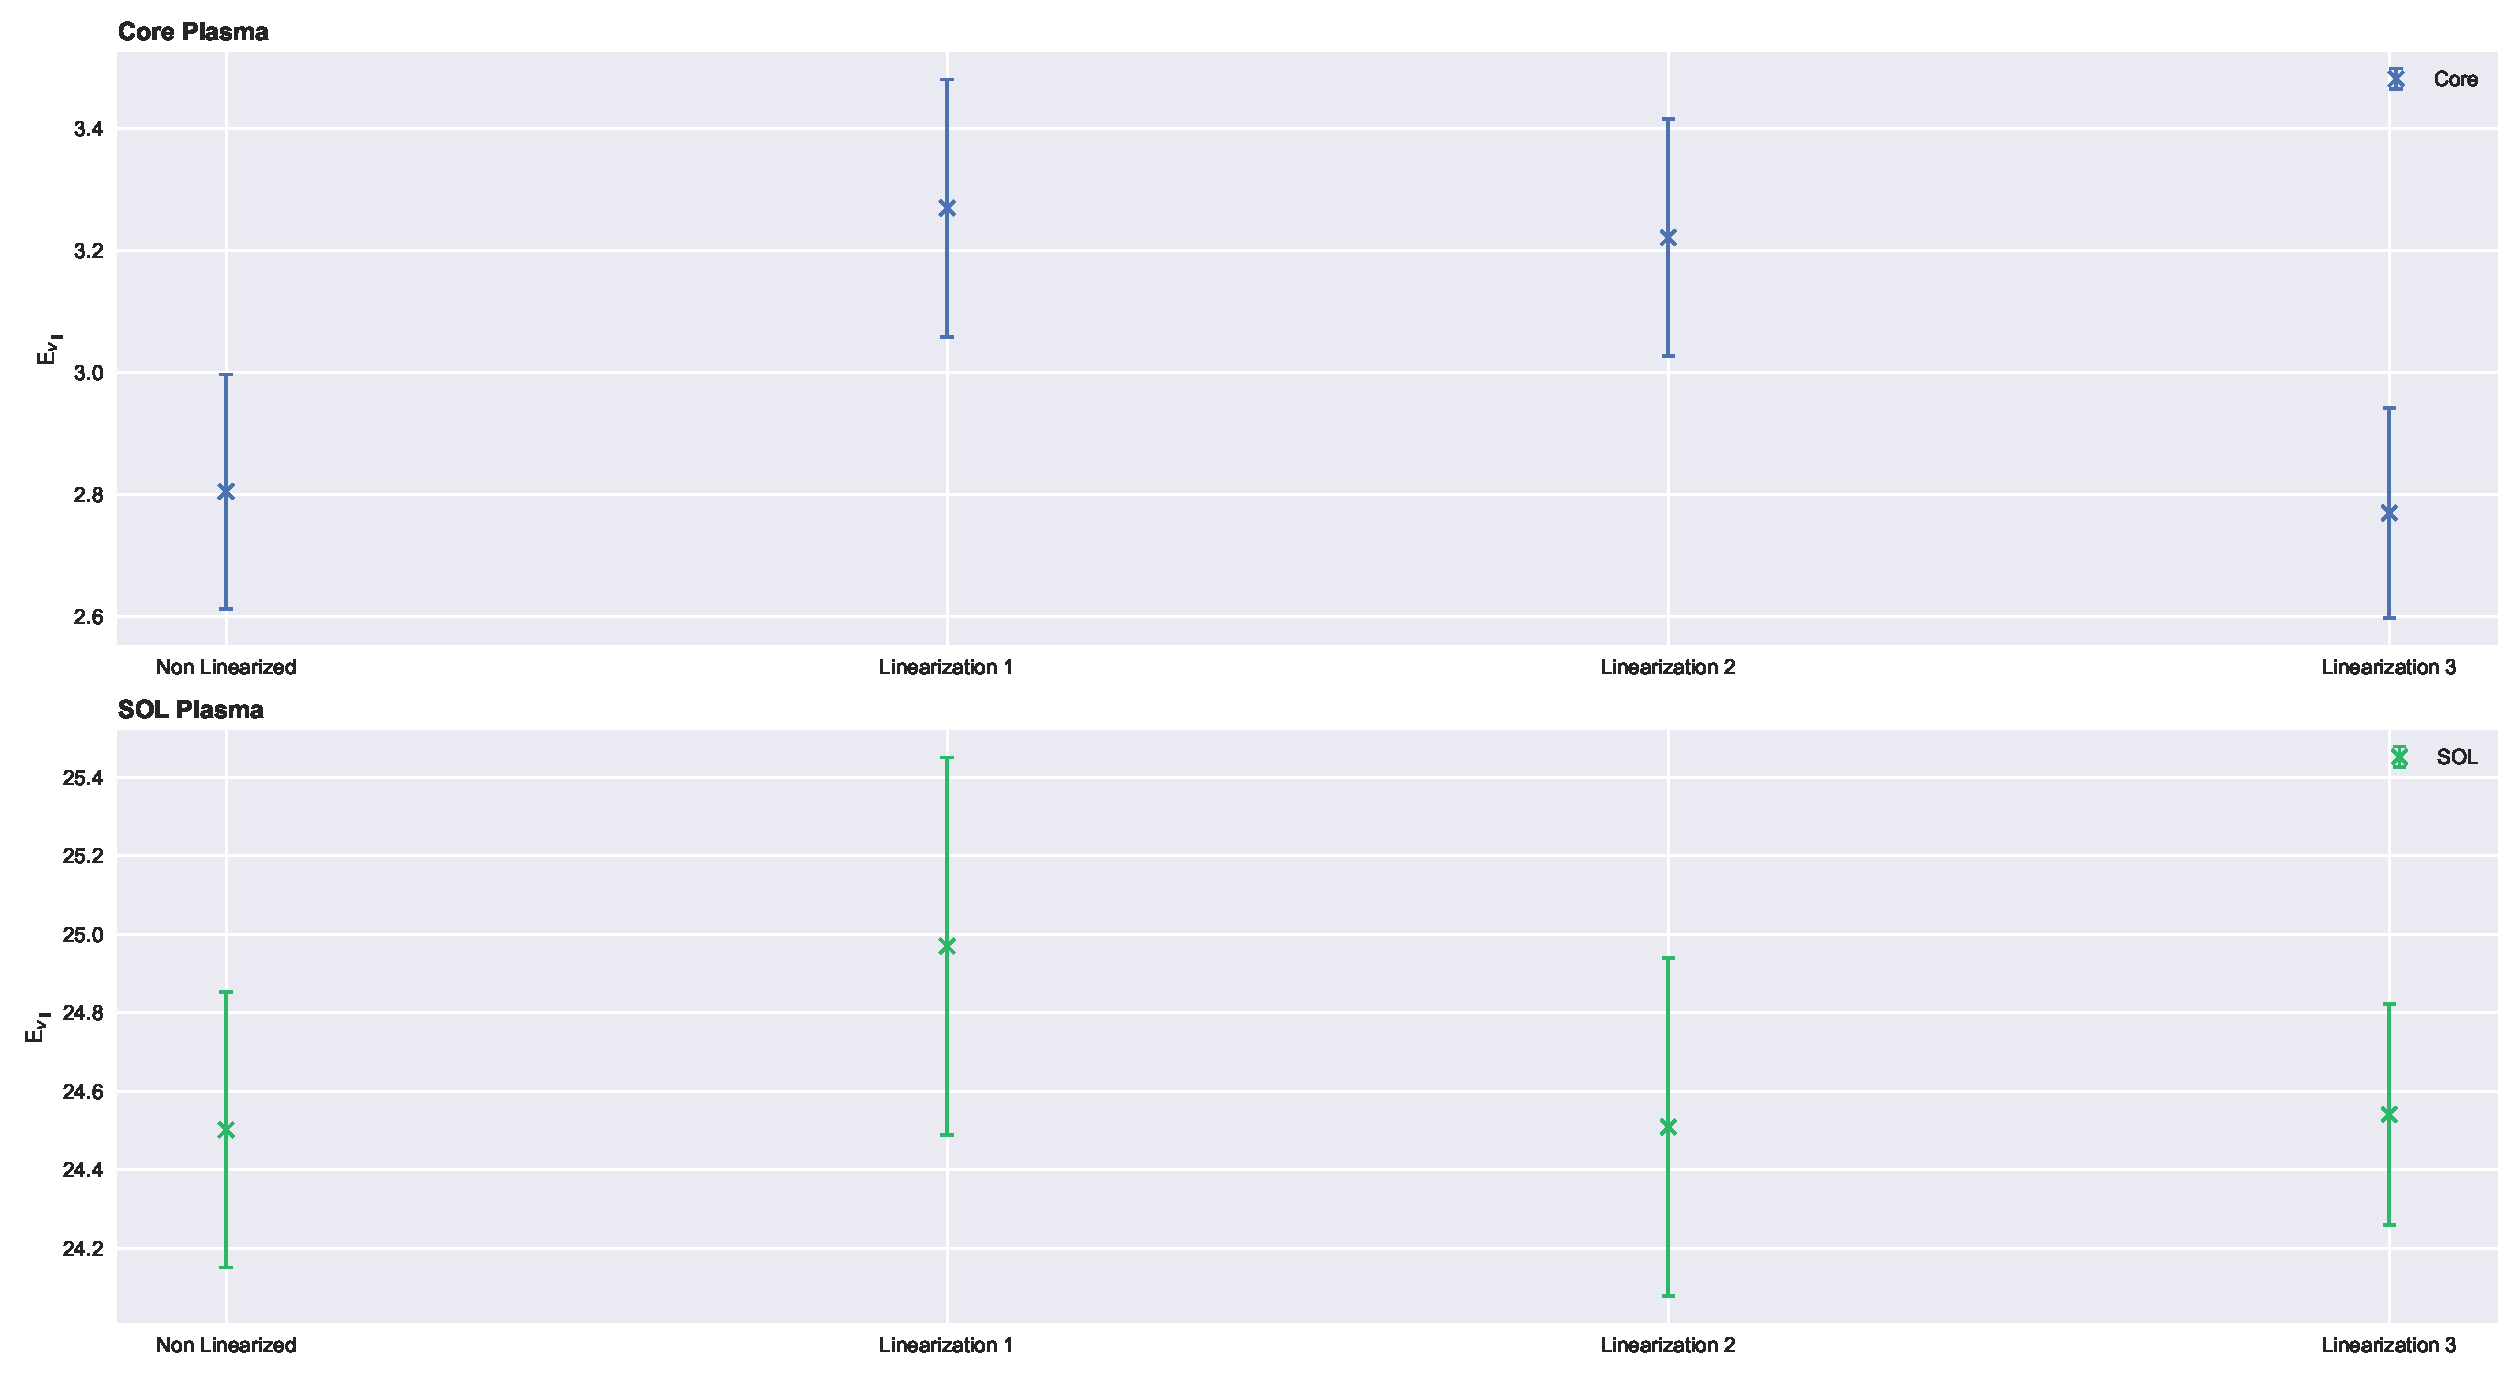
\includegraphics[width=\linewidth]{pdfs/velocity-energy-low-means.pdf}
    \caption{Mean of Velocity Energy from 80,000 to 200,000 iterations}
    \label{fig:velocity-energy-low-mean}
\end{figure}

\section{High resolution Data \textit{(2\textsuperscript{nd} parameter set)}}
The same procedures from the previous sections are applied to a finer grid (8x256x1024; $h_x = h_y = 0.5$). One has to account for a higher resolution by reducing $\Delta t$ to stay in the \ac{CFL} limit. It is also expected that the perpendicular viscosity has to be adjusted to account for the higher resolution in the perpendicular plane because the finer grid now allows higher wave numbers. \newline
\todo{Understand this derivation....}The perpendicular viscosity is realized using the fourth derivative in $x$ and $y$ direction.. \newline
To get a one to one mapping from the lower resolution to the higher resolution turned out to be very difficult because the higher resolution has a great negative impact on the stability. In the following sections two parameter sets are presented where the first tries to achieve a mapping from the lower resolution to the higher and the second one represents a new parameter set with higher viscosities.

\subsection{1\textsuperscript{st} Parameter Set High Resolution}
This parameter set should actually represent resolution scaling but to achieve a stable set it was necessary to reduce $\Delta t$ to $0.001$. Now it would have been necessary to run the simulation for a lot longer time but this was not done here because when looking at the data after 200,000 iterations numerical artifacts are already visible.\newline
For this set only $\Delta t$ and $\nu_\perp = 0.001375$ where changed.\newline
The mean values were taken from iteration 160,000 to 200,000.
\autoref{fig:density-velocity-high-wrong} shows the evolution of full density and velocity. Here one already sees that something unexpected is happening with linearization two. Also some kind of resonance is visible in the parallel kinetic energy. This probably arises from the small timestep for which the timestepper is not stable anymore.

\begin{figure}[!hbtp]
    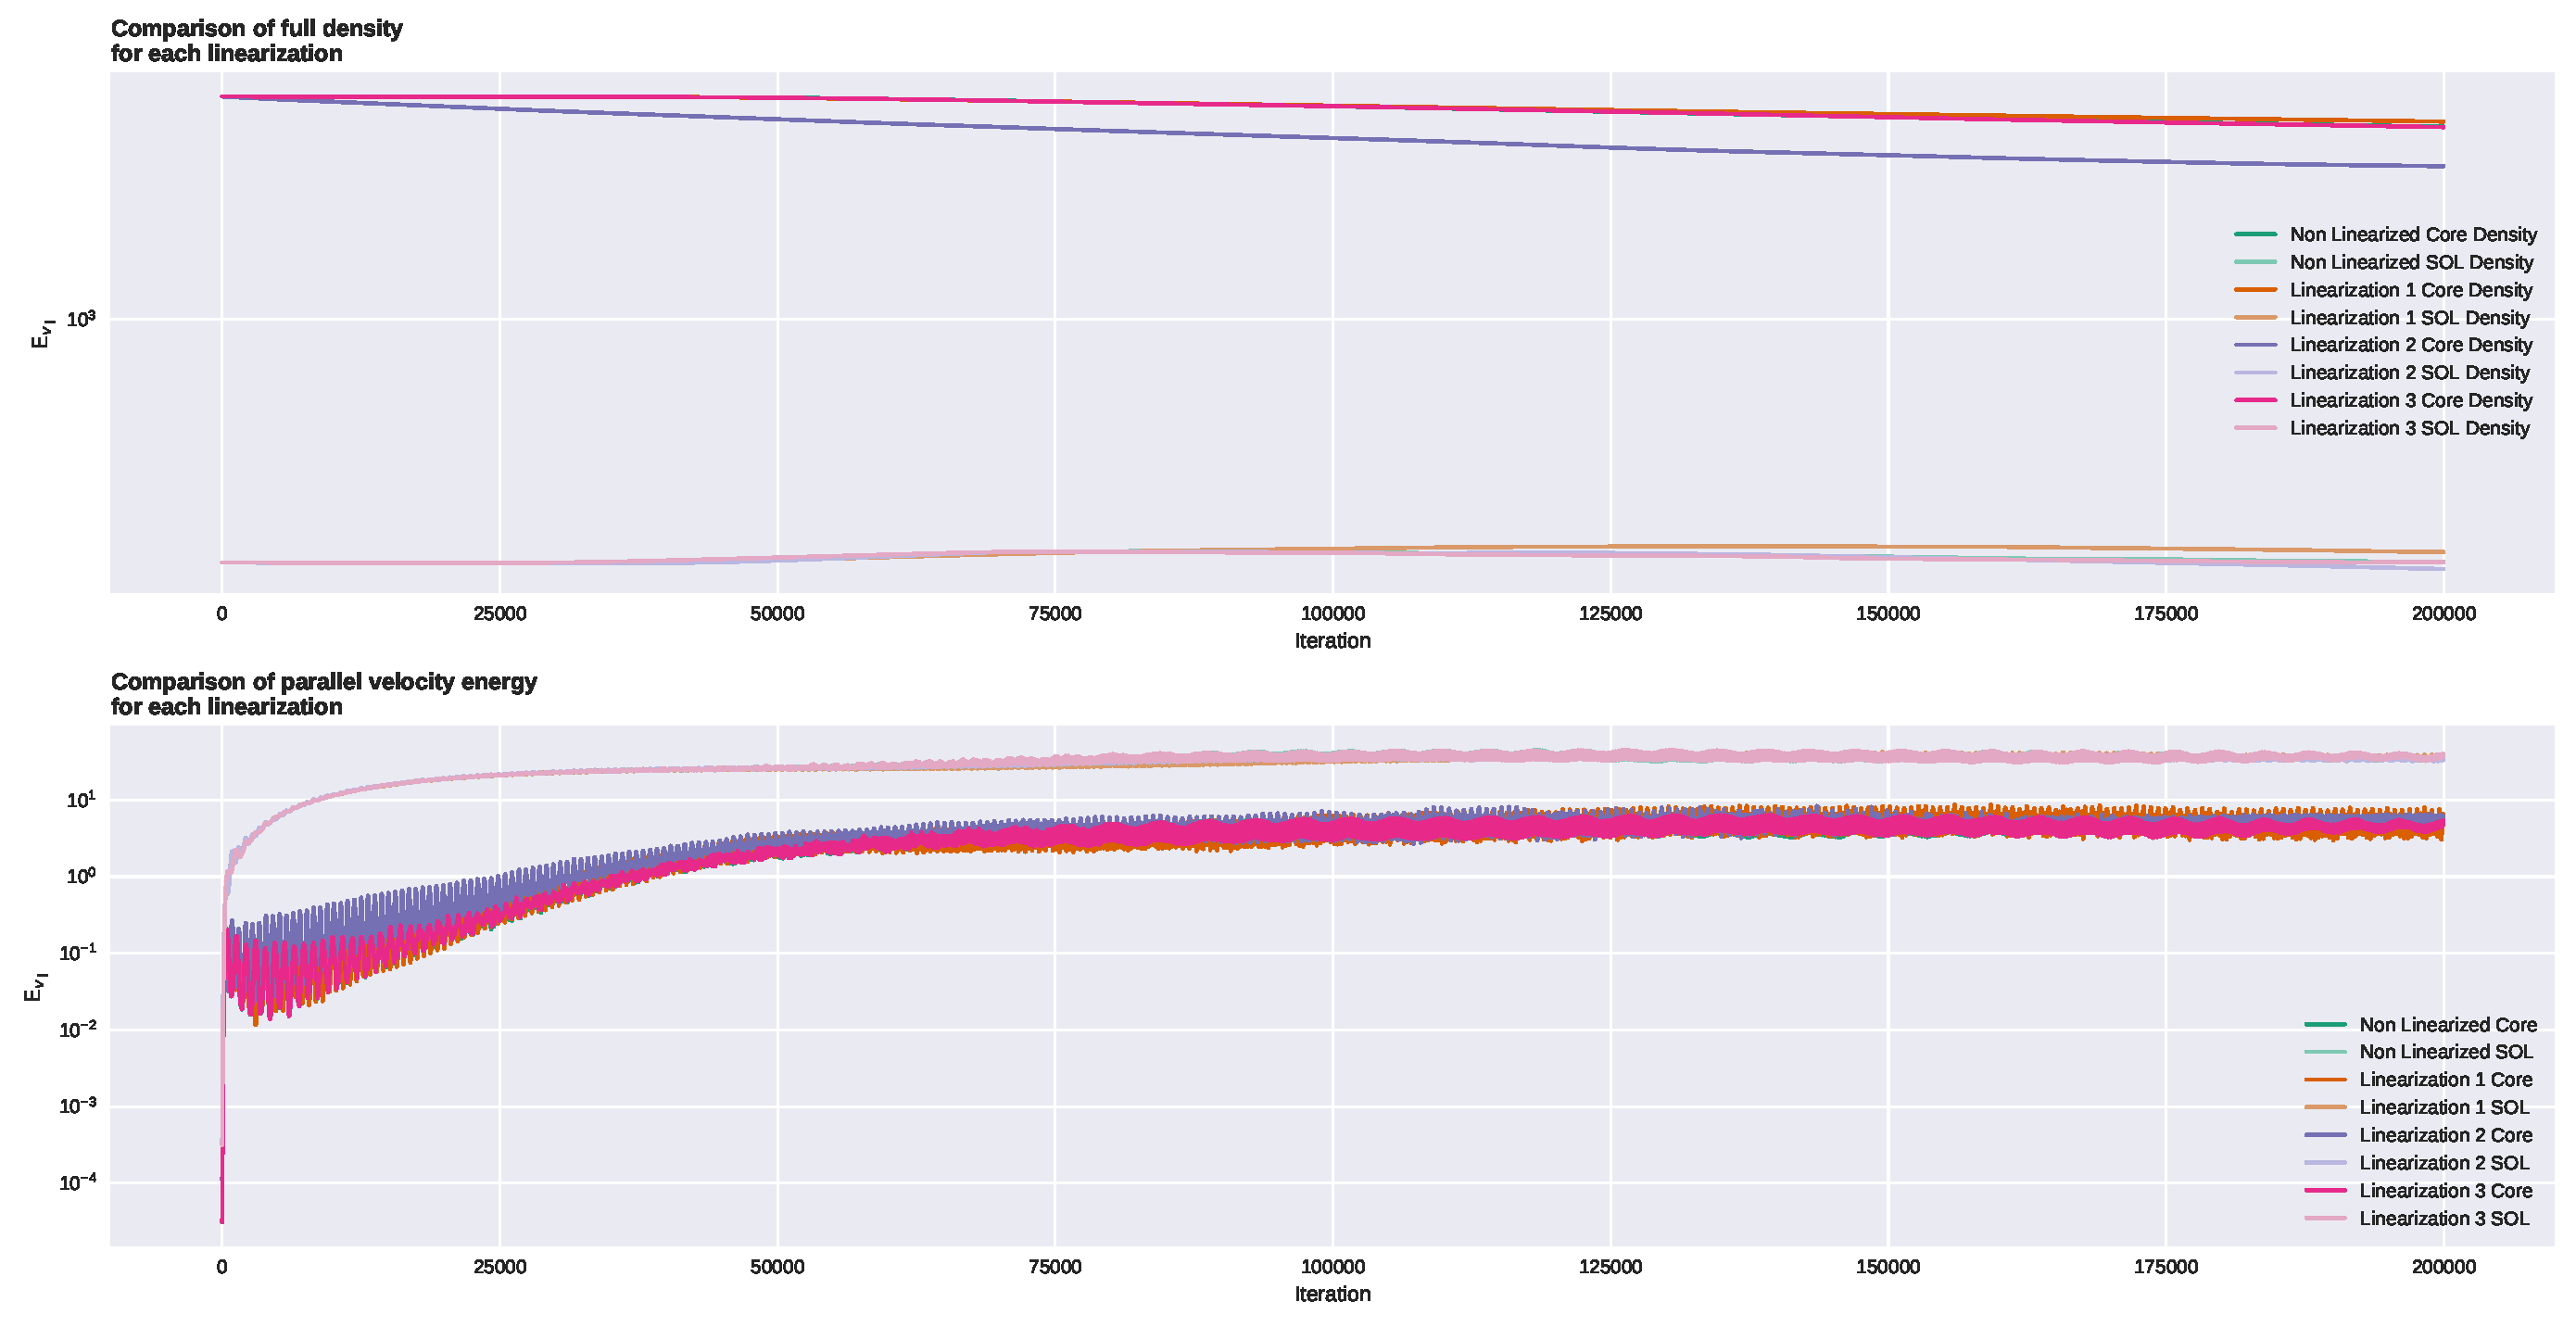
\includegraphics[width=\linewidth]{pdfs/0-11_0-001375/density_vs_velocity.pdf}
    \label{fig:density-velocity-high-wrong}
    \caption{Full density and parallel energy for the 1\textsuperscript{st} parameter set at a higher resolution.}
\end{figure}

\autoref{fig:zonal_profiles-high_wrong} shows the zonal profiles but here the outlier linearization two is clearly visible. Considering the instable nature of this parameter set it is discarded further on and was only presented to show the difficulties involved with resolution scaling for this model and simulation.

\begin{figure}[!hbtp]
    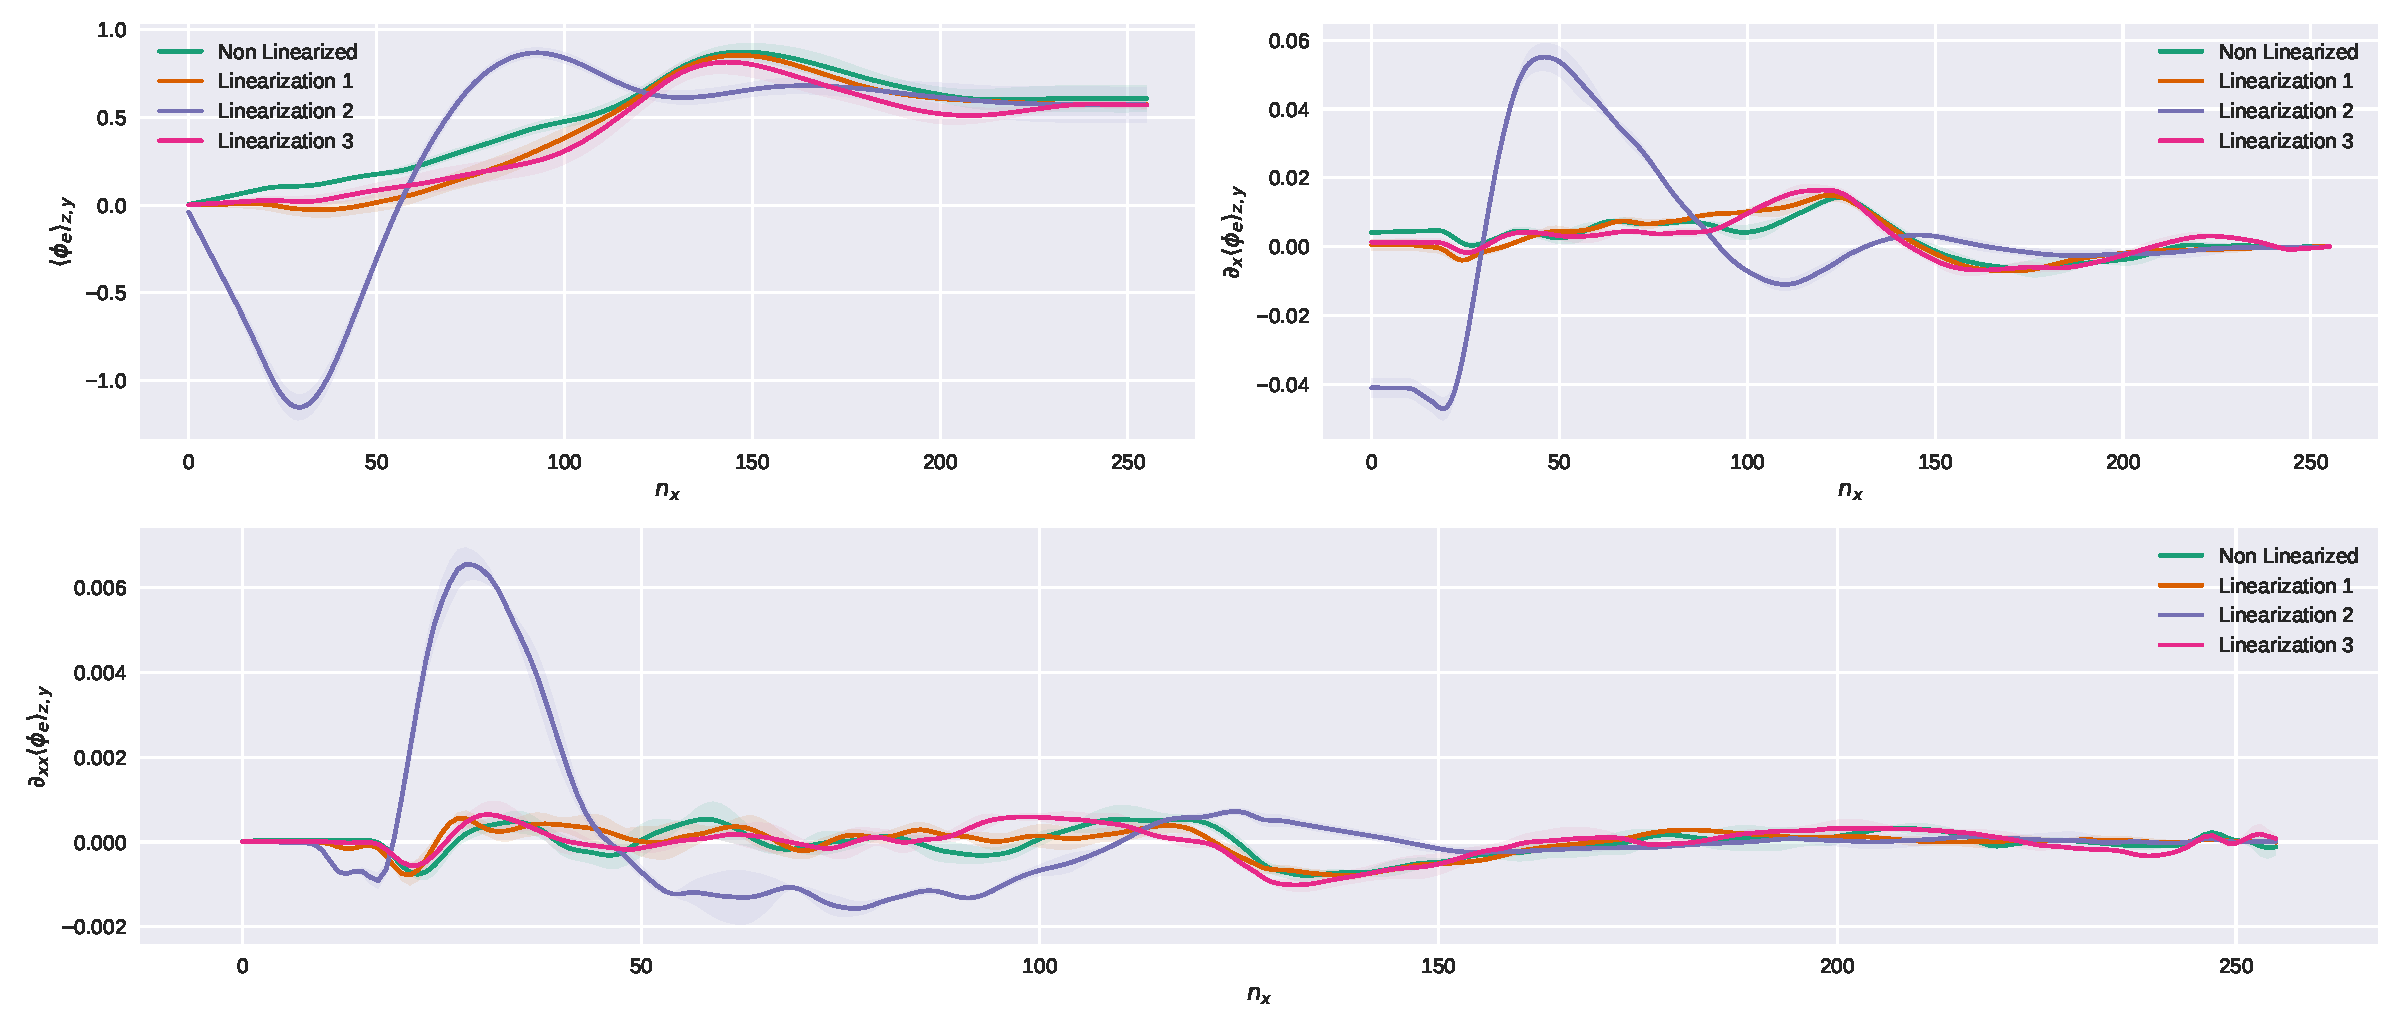
\includegraphics[width=\linewidth]{pdfs/0-11_0-001375/zonal_profiles.pdf}
    \label{fig:zonal_profiles-high_wrong}
    \caption{Zonal profiles for the 1\textsuperscript{st} parameter set at a higher resolution.}
\end{figure}

\subsection{2\textsuperscript{nd} Parameter Set}
A second parameter set was evaluated where $\nu_\parallel = 0.4$ and $\nu_\perp = 0.06$. These parameters produce a stable simulation for the higher resolution at $\Delta t = 0.01$. Only the zonal profiles (\autoref{fig:zonal_profiles-high_good}), values for the turbulent flow (\autoref{fig:turbulent-flow-means-high_good}) and the parallel kinetic energy (\autoref{fig:velocity-energy-means-high_good}) are presented here. 

\begin{figure}[!hbtp]
    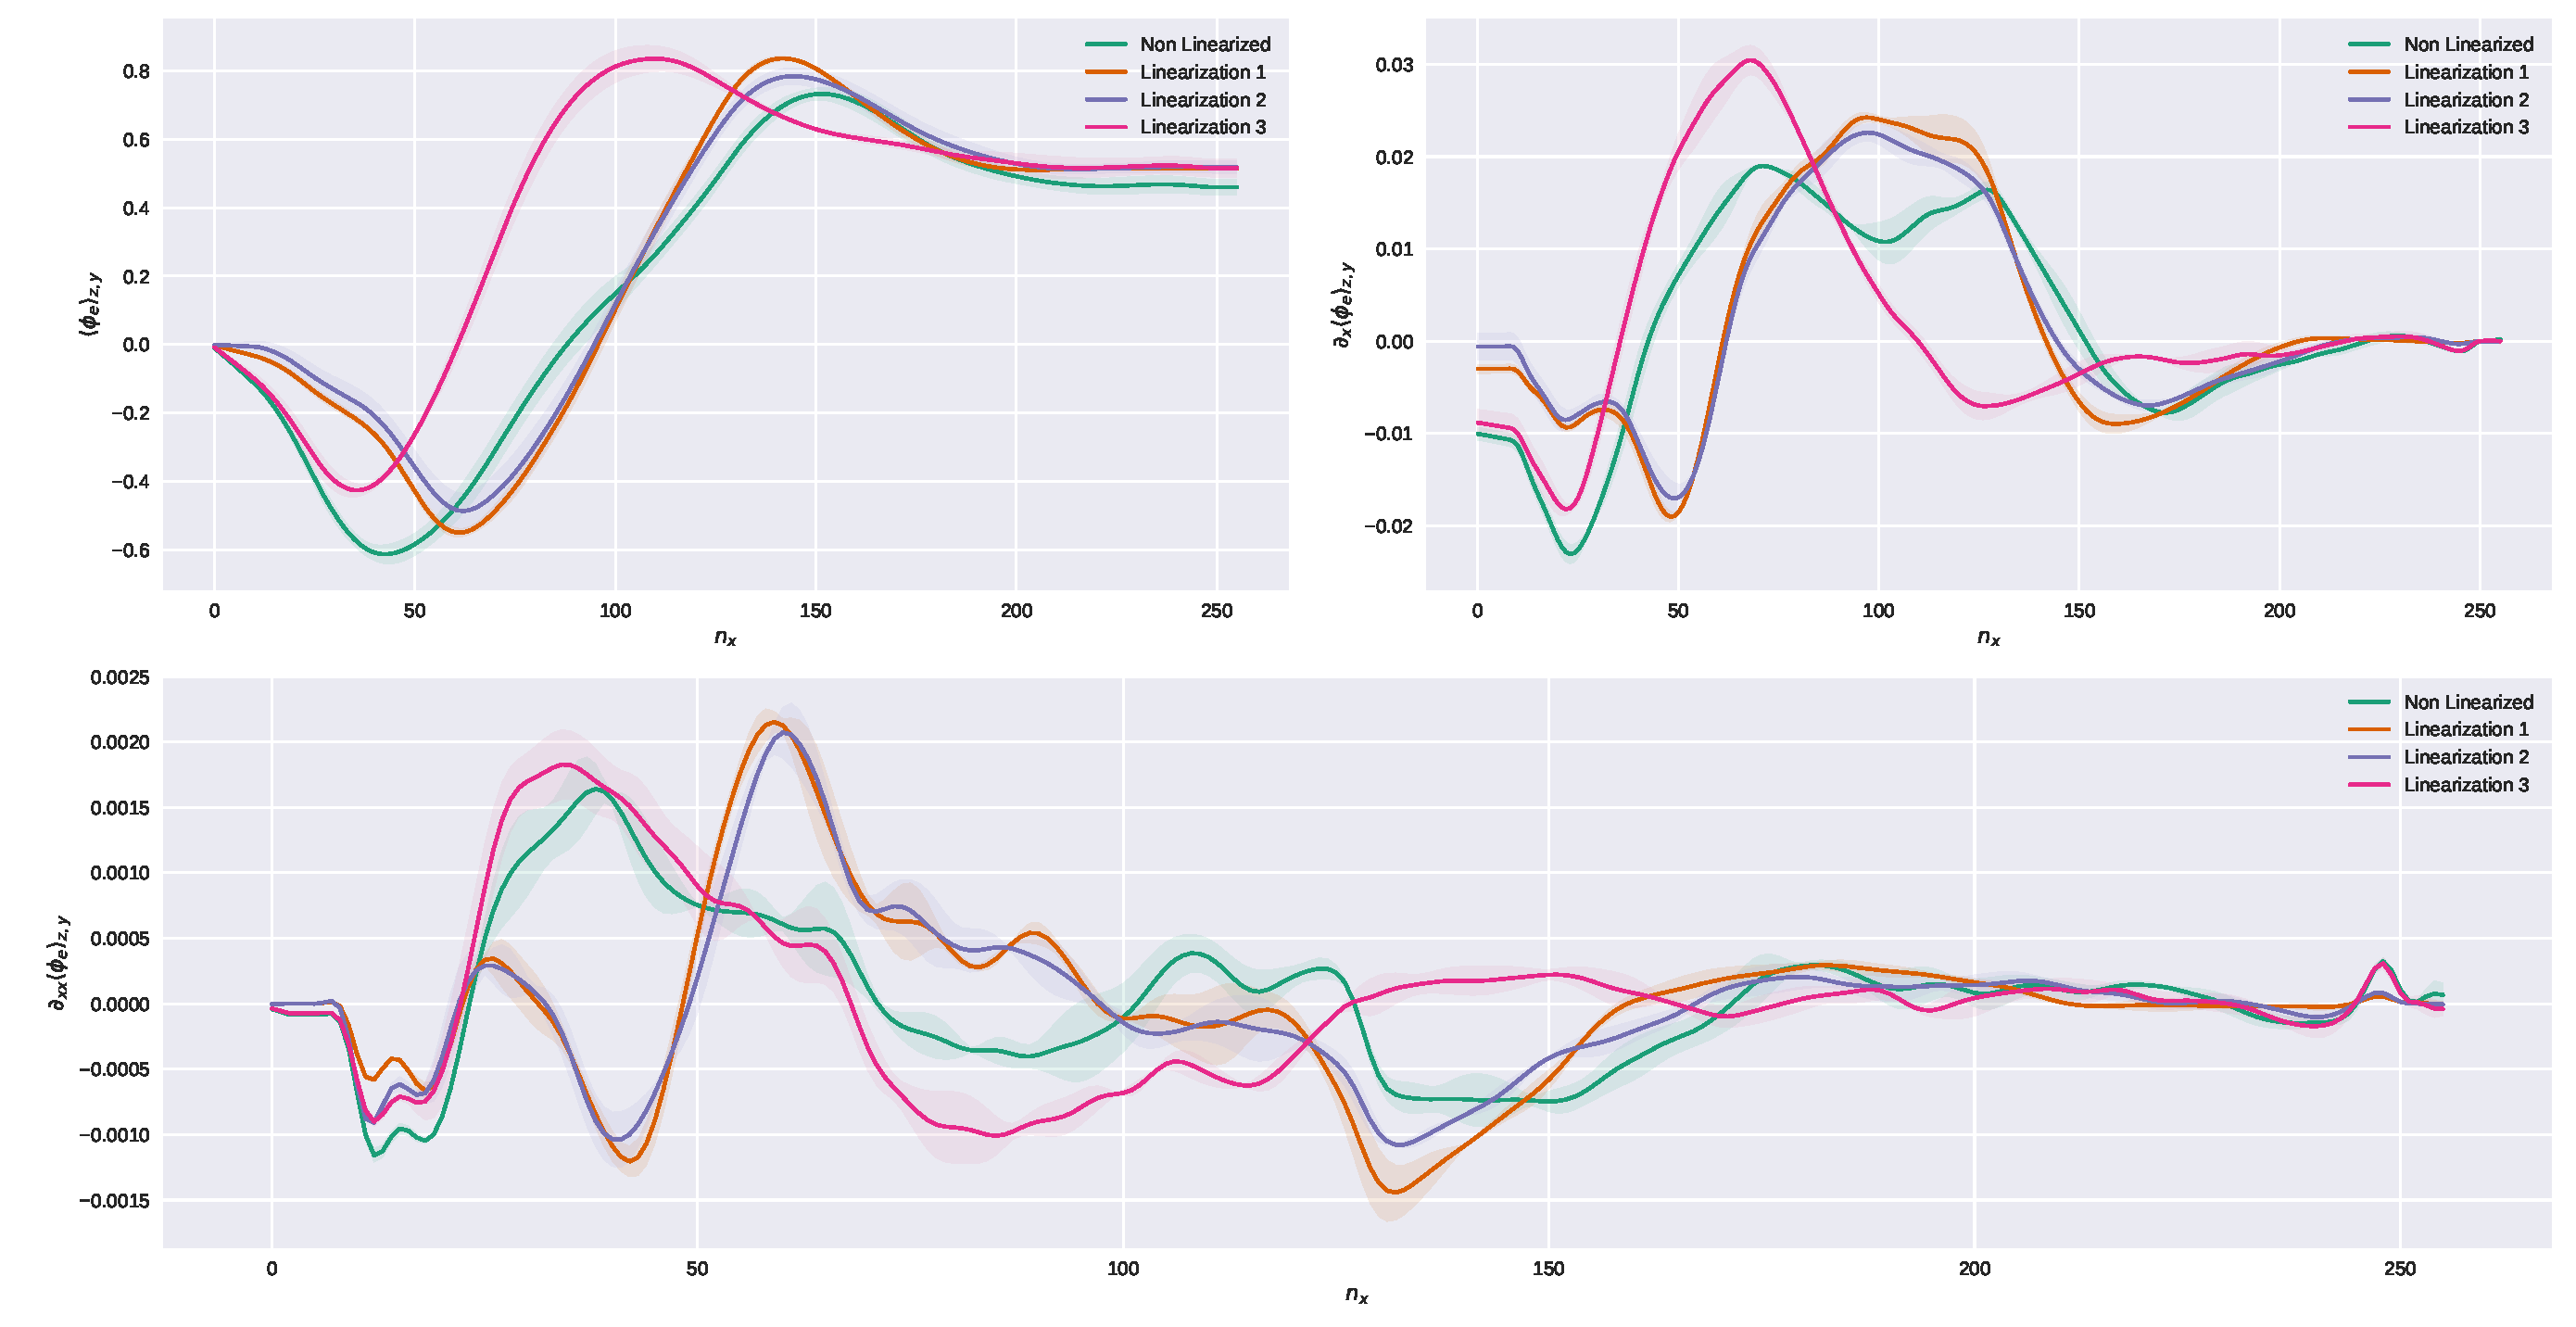
\includegraphics[width=\linewidth, height=150px]{pdfs/0-4_0-06/zonal_profiles.pdf}
    \caption{Zonal profiles for the 2\textsuperscript{nd} parameter set.}
    \label{fig:zonal_profiles-high_good}
\end{figure}

In this case the Zonal Potential profile shows a strongly differing behavior for linearization three. For Zonal Flow and Zonal Flow potential this has a strong effect on the region around the separatrix ($n_x\approx 128$). But excluding the Zonal Potential the two groups are visible again.

\begin{figure}[!hbtp]
    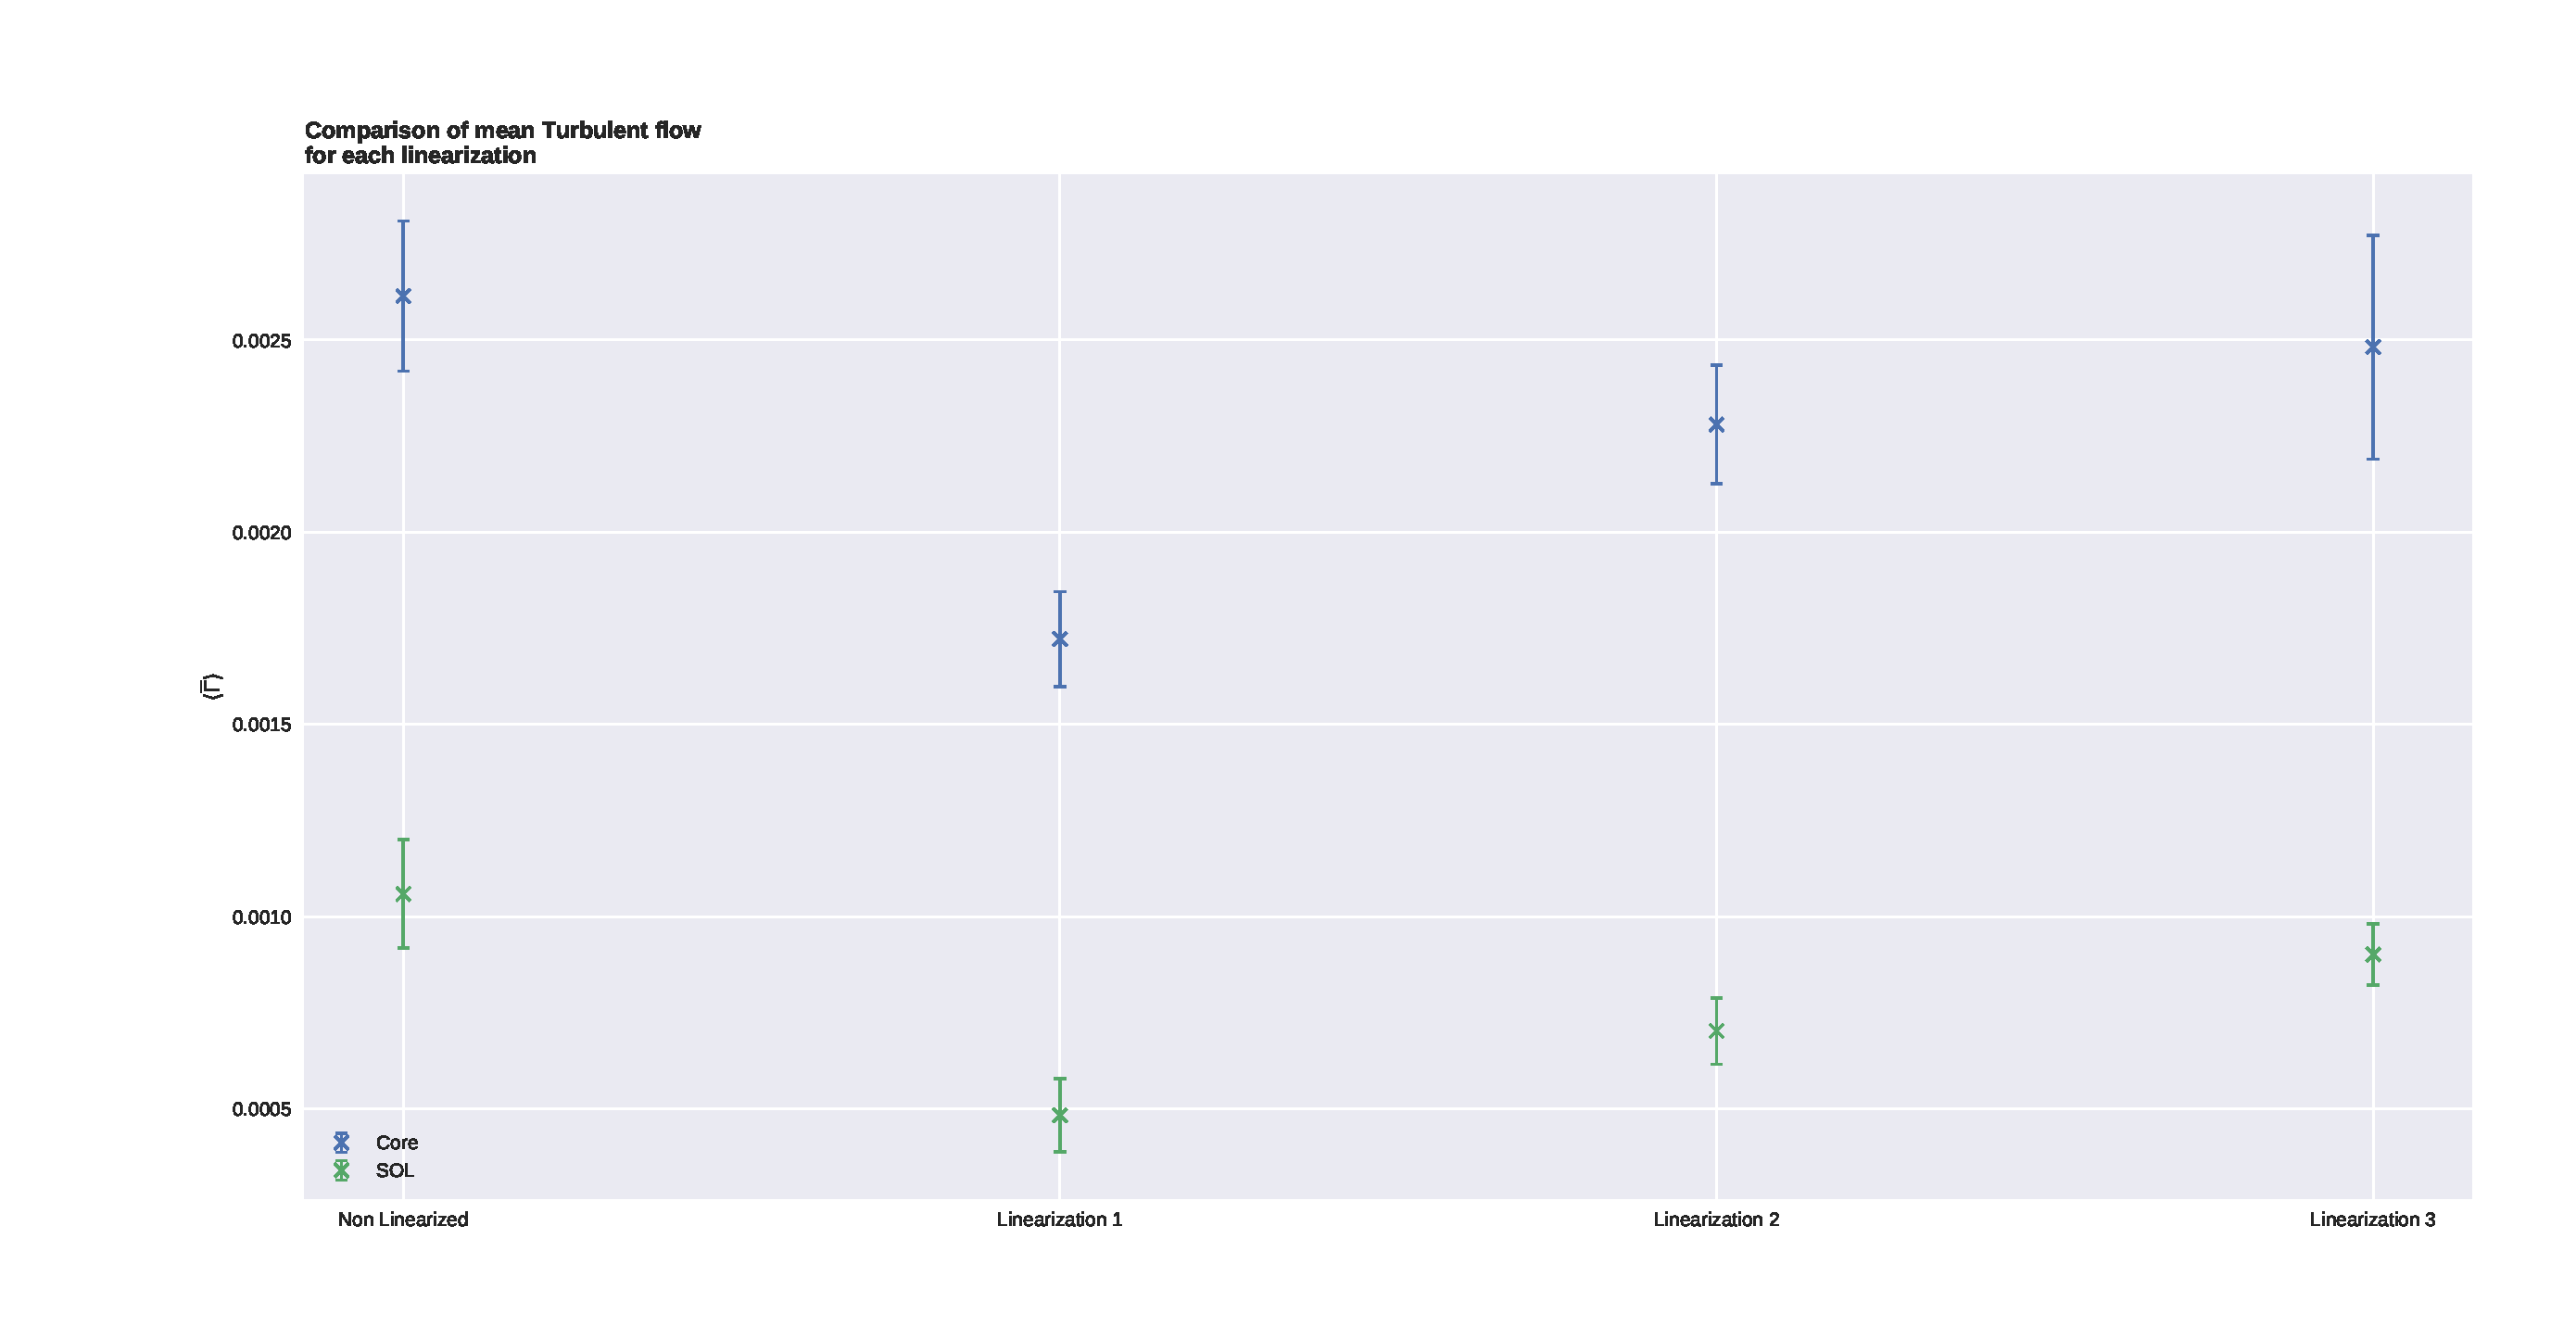
\includegraphics[width=\linewidth, height=150px]{pdfs/0-4_0-06/turbulent_flow_means.pdf}
    \caption{Mean of turbulent flow from iteration 160,000 to 200,000 for the 2\textsuperscript{nd} parameter set.}
    \label{fig:turbulent-flow-means-high_good}
\end{figure}

\begin{figure}[!hbtp]
    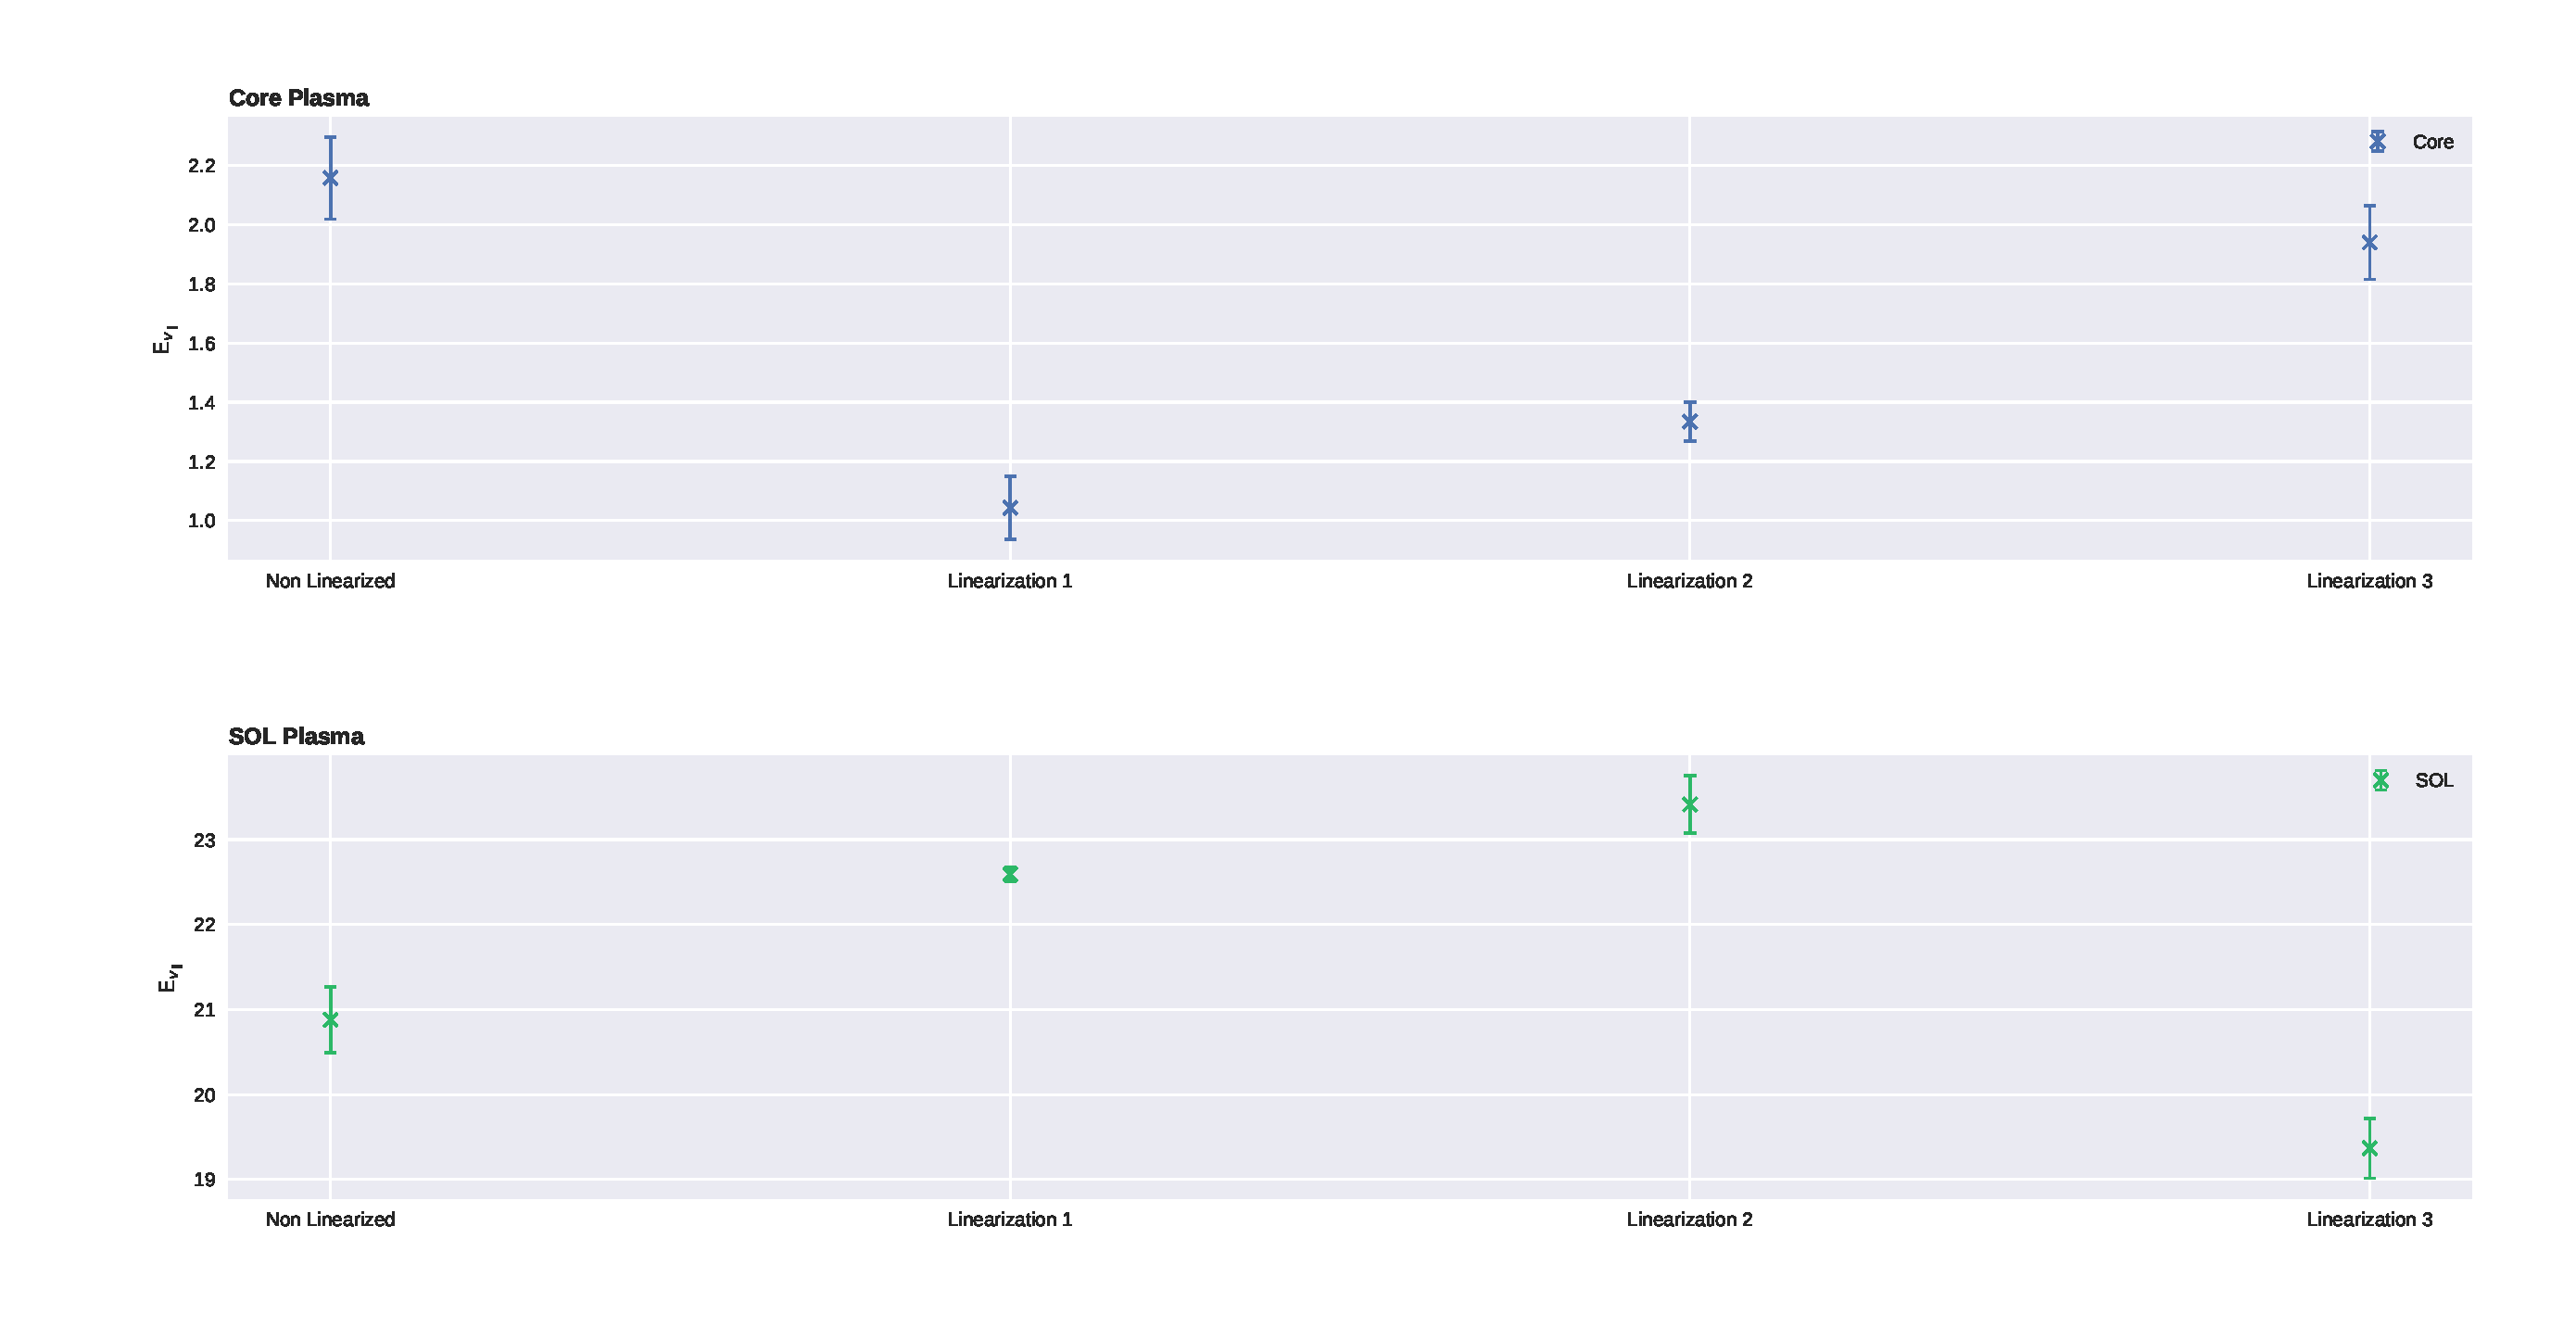
\includegraphics[width=\linewidth, height=150px]{pdfs/0-4_0-06/velocity_energy_means.pdf}
    \caption{Mean of parallel kinetic energy from iteration 160,000 to 200,000 for the 2\textsuperscript{nd} parameter set.}
    \label{fig:velocity-energy-means-high_good}
\end{figure}

When looking at the turbulent flow and the parallel kinetic energy an inversion in respect to the first parameter set happens where the first group now generates higher values and the second group generates lower values. Since this is strongly visible in the parallel kinetic energies this is most likely connected to the change of $\nu_\parallel$. Another option would be the change of resolution.\newline
For this parameter set the differences between the linearizations are generally more significant and for example the $\left< \overline{\Gamma} \right>$ in the Core region for the non linearized solver is double the magnitude of the linearization one.




\section{Numerical stability}
Not thoroughly measured was the stability of the simulation but still some information will be presented here. For example if one increases the magnetic curvature to 0.05 for the lower resolution grid (leading to stronger turbulence) only the non linearized model is numerical stable. One has to deal with high gradients at the boundaries which seem to be a greater problem for the linearized models. 
Furthermore if the resolution is increased the $\Delta t$ has to be decreased but the non linearized model is still stable for higher $\Delta t$'s whereas the linearizations are much more sensitive to an increase of the resolution and need smaller $\Delta t$'s. It seems that the \ac{CFL} number is higher for the linearized models.

\section{Conclusion}
In this chapter the different linearizations for the Poisson equation have been evaluated for two different parameter sets representing two different resolutions. The first set showed little change between the different linearizations and mostly effected the $x$-boundaries where the highest density gradients are present. There is a small tendency to lower turbulent flows which may be connected to a damping effect of the Debye-Shielding term which the linearizations target. There was also some evidence that the second group\footnote{Linearization 1 and 2} of linearizations is less stable (i. e. the simulation does not converge for a parameter set) than the first group\footnote{Non linearized and 3rd Linearization} which may also suggest a dampening effect. The dampening could slow down the \textit{velocity of change} of for instance density fluctuations and thus reduce the \ac{CFL}-number leading to a more stable simulation. Another possibility could be the higher Zonal-Flow for the second group that may suppress higher gradients in $y$-direction via an increased mixing and thus faster destruction of strong instabilities \footnote{Generally the solver converges worse for higher gradients.}. This should be investigated further by analyzing parameter sets where the second group does not converge but the first does.
Scaling the first parameter set to a higher resolution was not possible since the simulation became unstable. Therefore a second parameter set at a higher resolution was evaluated where the viscosities where chosen higher. This produced somewhat different results than the first parameter set. The differences between the two groups became larger and the non linearized case did not coincide worse with the third linearization. Where this effect stems from can not be deduced from the two sets. It could either be the higher resolution or the impact of the very different viscosities but it shows that the influence of the linearizations is not obvious.\newline



\end{document}